\documentclass[a4paper]{elsarticle}
\usepackage[utf8]{inputenc}
\usepackage[T1]{fontenc}
%\usepackage[spanish]{babel}
\usepackage{amsmath}
\usepackage{amsfonts}
\usepackage{amssymb}
\usepackage{graphicx}
\usepackage{mathtools,amssymb}
\usepackage{subfigure}
\usepackage{optidef}
\usepackage{xcolor}
\usepackage{amsthm}
\usepackage{comment}
\usepackage{tikz}
\usepackage{pgfplots}
\usepackage{mathrsfs}
\usepackage{float}
\usepackage[linesnumbered,ruled,vlined]{algorithm2e}
%\usepackage[noend]{algpseudocode}
%\usepackage{ulem}
\usepackage[margin=1in]{geometry}
\usepackage{enumitem}
\usepackage{xspace}
\usepackage{array}
\setlength{\extrarowheight}{.5ex}


\usepackage{threeparttable}

\usepackage[utf8]{inputenc}

\title{The Traveling Postman Problem with Linear Barriers}
\author{carlosvalverdemartin-y-otro}
\date{February 2021}

\DeclareMathOperator*{\argmax}{arg\,max}
\DeclareMathOperator*{\argmin}{arg\,min}


\newcommand{\SPPN}{{\sf{H-SPPN}\xspace }}
\newcommand{\TSPN}{{\sf{H-TSPN}\xspace }}
\newcommand{\TSPVN}{{\sf{H-TSPVN}\xspace }}
\newcommand{\B}{{\mathcal B}}
\newcommand{\VB}{{V^{}_{\mathcal B}}}
\newcommand{\EB}{{E^{}_{\mathcal B}}}
\newcommand{\VS}{{V^{}_{S}}}
\newcommand{\ES}{{E^{}_{S}}}
\newcommand{\VT}{{V^{}_{T}}}
\newcommand{\ET}{{E^{}_{T}}}
\newcommand{\VN}{{V^{}_{\mathcal N}}}
\newcommand{\EN}{{E^{}_{\mathcal N}}}

\newtheorem{remark}{Remark}
\newtheorem{notation}{Notation}

\newtheorem{prop}{Proposition}

\definecolor{armygreen}{rgb}{0.19, 0.53, 0.43}
\definecolor{atomictangerine}{rgb}{1.0, 0.6, 0.4}
\newcommand{\JP}[1]{{\color{armygreen}#1}}
\newcommand{\CV}[1]{{\color{atomictangerine}#1}}


\begin{document}

\maketitle
	\section{Description of the Problems}\label{section:description}
	This section describes the two problems that are considered in this paper: the Hampered Shortest Path Problem with Neighborhoods \SPPN \ and the Hampered Traveling Salesman Problem with Neighborhoods \TSPN. In both models, we state the following assumptions:
	
	\begin{enumerate}[label=\textbf{A\arabic*},ref=\textbf{A\arabic*}]
		\item \label{A1}The line segments of $\mathcal B$ are located in general position, i.e., the endpoints of these segments are not aligned. Although it is possible to model the most general case, \JP{one can always to slightly modify one of the endpoints so that the segments are in general position.}
		\item The line segments of $\mathcal B$ are opened, that is, it is possible that the drone visits  endpoints of segments, but entering  in the interior points of them is not allowed. \JP{Observe that without loss of generality, we can always slightly enlarge these segments to make them opened.}
		\item If there are two barriers that have a common portion of them, it is only considered the smallest line segment that contains both barriers.
		\item \label{A4}There is no a rectilinear path to go from $N_S$ to $N_T$. Otherwise, the problem becomes straightforward and the solution is the minimum distance between both neighborhoods.
	\end{enumerate}
	
	%In \SPPN, we have a source neighborhood $N_S\subset\mathbb R^2$ and a target neighborhood $N_T\subset\mathbb R^2$, that we assume to be convex sets and a set $\mathcal B$ of opened line segments located in general position that plays the role of barriers that the drone cannot cross, i.e., the drone can visit the endpoints of these barriers but it cannot be located in the interior points of the barriers. Note that, it is rational to assume that if there are two barriers that have a portion of them in common, it is only considered the smallest line segment that contains both barriers. The aim of the \SPPN is to find the best pair of points $(P_{S}, P_{T})\in N_S\times N_T$ in the source and target neighborhoods that minimize the length of the path that joins both points without crossing any barrier of $\mathcal B$. In this problem, it is implicitly assumed that there is not a rectilinear path to go from $N_S$ to $N_T$, otherwise, the problem becomes straightforward and the solution is the minimum distance between both neighborhoods. 
	
	\subsection{Description of the Hampered Shortest Path Problem with Neighborhoods}\label{subsection:descriptionHSPPN}
	In \SPPN, we have a source neighborhood $N_S\subset\mathbb R^2$ and a target neighborhood $N_T\subset\mathbb R^2$, that we assume to be second order cone representable sets and a set $\mathcal B$ of line segments that play the role of barriers that the drone cannot cross. 
	
	The aim of the \SPPN \ is to find the best pair of points $(P_{S}, P_{T})\in N_S\times N_T$ in the source and target neighborhoods that minimize the length of the path that joins both points without crossing any barrier of $\mathcal B$ and assuming \ref{A1}-\ref{A4}. To state the model,  we define the following sets:
	\begin{itemize}
		\item $\VS=\{P_S\}$: set composed by the point selected in the source neighborhood $N_S$.
		\item $\VB=\{P^1_B, P^2_B:B=\overline{P^1_B P^2_B}\in \mathcal B\}$: set of vertices that come from the endpoints of barriers in the problem.
		\item $\VT=\{P^{}_T\}$: set composed by the point selected in the target neighborhood $N_T$.
		\item $\ES=\{(P_S, P^i_{B}):P^i_B\in V_\B\text{ and } \overline{P_SP^i_B}\cap B''=\emptyset,\forall B''\in\B,\:i=1,2\}$: set of edges formed by the line segments that join the point selected in the source neighborhood and every endpoint in the barriers that do not cross any barrier in $\B$.
		\item $\EB=\{(P^{i}_B, P^{j}_{B'}):P^i_B, P^j_{B'}\in \VB \text{ and } \overline{P^i_B P^j_{B'}}\cap B''=\emptyset,\:\forall B''\in\mathcal B,\:i, j=1,2\}$: set of edges formed by the line segments that join two vertices of $V_{\mathcal B}$ and do not cross any barrier in $\B$.
		\item $\ET=\{(P^i_{B}, P^{}_T):P^i_B\in V_\B\text{ and } \overline{P^i_BP^{}_T}\cap B''=\emptyset,\forall B''\in\B,\:i=1,2\}$: set of edges formed by the line segments that join the point selected in the target neighborhood and every endpoint in the barriers that do not cross any barrier in $\B$.
	\end{itemize} 
	
	At this point, we can define the graph $G= (V, E)$ induced by the barriers and neighborhoods, where $V=\VS\cup \VB\cup\VT$ and $E=\ES\cup\EB \cup\ET$. It is interesting to note that this graph can be split into two parts: a fixed graph $G_\B=(\VB,\EB)$ whose edges can be computed by using the Remark \ref{rem:determinants} and the sets $\VS$, $\ES$, $\VT$ and $\ET$ that depend on where the points $P_S$ and $P^{}_T$ are located as shown in Figure \ref{fig:graph}.  The figures show how the graph $G$ is generated. The blue dashed line segments represent the edges of $\ES$, the green ones, the edges of $\ET$ and the red dashed lines, the edges of $\EB$. A special case that can be remarked occurs when the neighborhoods are points. In that case, the induced graph is completely fixed and it is only necessary to find which edges are included by keeping in mind that there can not have crossings. This idea is exploited in Subsection \ref{section:reformulation}.
	
	%\textcolor{red}{Me estoy dando cuenta que nos pueden decir que para qué tenemos en cuenta todo el conjunto si realmente se pueden coger los puntos de la frontera mas cerca a cada uno de los puntos por donde puede salir de las barreras. Es cierto que solo ocurre con el SPP. En el caso del TSP esto no es cierto.}
	
	\pgfplotsset{compat=1.15}
\usetikzlibrary{arrows}
\begin{figure}[h!]
\centering
\definecolor{qqffqq}{rgb}{0,1,0}
\definecolor{qqqqff}{rgb}{0,0,1}
\definecolor{ffqqqq}{rgb}{1,0,0}
\begin{tikzpicture}[line cap=round,line join=round,>=triangle 45,x=1cm,y=1cm, scale=0.65]
\begin{axis}[
x=0.1cm,y=0.1cm,
axis lines=middle,
xmin=-5,
xmax=105,
ymin=-5,
ymax=105,
xtick={-30,-20,...,160},
ytick={-30,-20,...,100},]
\clip(-30.537729395742623,-31.914778968980123) rectangle (160.8609499148995,105.01143884235292);
\draw [line width=1pt,color=ffqqqq] (20,80)-- (40,30);
\draw [line width=1pt,color=ffqqqq] (70,95)-- (40,70);
\draw [line width=1pt,color=ffqqqq] (95,60)-- (60,70);
\draw [line width=1pt,color=ffqqqq] (60,50)-- (90,10);
\draw [line width=1pt,color=ffqqqq] (10,70)-- (20,50);
\draw [line width=1pt,dashed,color=ffqqqq] (10,70)-- (20,80);
\draw [line width=1pt,dashed,color=ffqqqq] (20,50)-- (40,30);
\draw [line width=1pt,dashed,color=ffqqqq] (90,10)-- (40,30);
\draw [line width=1pt,dashed,color=ffqqqq] (20,80)-- (40,70);
\draw [line width=1pt,dashed,color=ffqqqq] (20,80)-- (70,95);
\draw [line width=1pt,dashed,color=ffqqqq] (40,70)-- (40,30);
\draw [line width=1pt,dashed,color=ffqqqq] (40,70)-- (60,70);
\draw [line width=1pt,dashed,color=ffqqqq] (70,95)-- (95,60);
\draw [line width=1pt,dashed,color=ffqqqq] (95,60)-- (90,10);
\draw [line width=1pt,dashed,color=ffqqqq] (60,50)-- (40,30);
\draw [line width=1pt,dashed,color=ffqqqq] (40,30)-- (60,70);
\draw [line width=1pt,dashed,color=ffqqqq] (60,70)-- (70,95);
\draw [line width=1pt,dashed,color=ffqqqq] (20,50)-- (20,80);
\draw [rotate around={0:(20,10)},line width=1pt,color=qqqqff,fill=qqqqff,fill opacity=0.25] (20,10) ellipse (1cm and 1cm);
\draw [rotate around={0:(90,90)},line width=1pt,color=qqffqq,fill=qqffqq,fill opacity=0.25] (90,90) ellipse (0.5cm and 0.5cm);
\draw [line width=1pt,dashed,color=ffqqqq] (10,70)-- (40,30);
\draw [line width=1pt,dashed,color=ffqqqq] (60,50)-- (60,70);
\draw [line width=1pt,dashed,color=ffqqqq] (60,50)-- (95,60);
\draw [line width=1pt,dashed,color=ffqqqq] (90,10)-- (60,70);
\draw [line width=1pt,dashed,color=qqqqff] (12.786085173820345,16.92527493177169)-- (10,70);
\draw [line width=1pt,dashed,color=qqqqff] (12.786085173820345,16.92527493177169)-- (20,50);
\draw [line width=1pt,dashed,color=qqqqff] (12.786085173820345,16.92527493177169)-- (40,30);
\draw [line width=1pt,dashed,color=qqqqff] (12.786085173820345,16.92527493177169)-- (90,10);
\draw [line width=1pt,dashed,color=qqffqq] (89.83150923646912,88.53724455912725)-- (70,95);
\draw [line width=1pt,dashed,color=qqffqq] (89.83150923646912,88.53724455912725)-- (40,70);
\draw [line width=1pt,dashed,color=qqffqq] (89.83150923646912,88.53724455912725)-- (60,70);
\draw [line width=1pt,dashed,color=qqffqq] (89.83150923646912,88.53724455912725)-- (95,60);
\draw [color=qqqqff](3.9007872968296593,8.815389811658244) node[anchor=north west] {$\mathbf{N_S}$};
\draw [color=qqffqq](95.46088215737039,101.20333363115502) node[anchor=north west] {$\mathbf{N_T}$};
\draw (87.18239256780974,95.5) node[anchor=north west] {$\mathbf{P_T}$};
\draw (5.722055006533001,19.742996069878295) node[anchor=north west] {$\mathbf{P_S}$};
\draw [line width=1pt,dashed,color=ffqqqq] (40,70)-- (60,50);
\draw [line width=1pt,dashed,color=ffqqqq] (60,50)-- (20,80);
\draw [line width=1pt,dashed,color=ffqqqq] (20,80)-- (90,10);
\draw [color=ffqqqq](68.5,53.8) node[anchor=north west] {$\mathbf{G_{\mathcal B}=(V_{\mathcal B}, E_{\mathcal B})}$};
\draw [color=qqffqq](68,90.11015758114377) node[anchor=north west] {$\mathbf{E_T}$};
\draw [color=qqqqff](21.1200456431158,33.9819981639226) node[anchor=north west] {$\mathbf{E_S}$};
\draw [line width=1pt,dashed,color=ffqqqq] (40,70)-- (95,60);
\draw [line width=1pt,dashed,color=ffqqqq] (40,70)-- (90,10);
\draw [line width=1pt,dashed,color=ffqqqq] (40,30)-- (70,95);
\begin{scriptsize}
\draw [color=ffqqqq] (20,80) circle (2.5pt);
\draw [color=ffqqqq] (40,30) circle (2.5pt);
\draw [color=ffqqqq] (70,95) circle (2.5pt);
\draw [color=ffqqqq] (40,70) circle (2.5pt);
\draw [color=ffqqqq] (95,60) circle (2.5pt);
\draw [color=ffqqqq] (60,70) circle (2.5pt);
\draw [color=ffqqqq] (60,50) circle (2.5pt);
\draw [color=ffqqqq] (90,10) circle (2.5pt);
\draw [color=ffqqqq] (10,70) circle (2.5pt);
\draw [color=ffqqqq] (20,50) circle (2.5pt);
\draw [fill=qqqqff] (12.786085173820345,16.92527493177169) circle (2.5pt);
\draw [fill=qqffqq] (89.83150923646912,88.53724455912725) circle (2.5pt);
\end{scriptsize}
\end{axis}
\end{tikzpicture}
\begin{tikzpicture}[line cap=round,line join=round,>=triangle 45,x=1cm,y=1cm, scale=0.65]
\begin{axis}[
x=0.1cm,y=0.1cm,
axis lines=middle,
xmin=-5,
xmax=105,
ymin=-5,
ymax=105,
xtick={-30,-20,...,160},
ytick={-30,-20,...,95},]
\clip(-30.537729395742623,-36.63351803502969) rectangle (160.8609499148995,109.73017790840248);
\draw [line width=1pt,color=ffqqqq] (20,80)-- (40,30);
\draw [line width=1pt,color=ffqqqq] (70,95)-- (40,70);
\draw [line width=1pt,color=ffqqqq] (95,60)-- (60,70);
\draw [line width=1pt,color=ffqqqq] (60,50)-- (90,10);
\draw [line width=1pt,color=ffqqqq] (10,70)-- (20,50);
\draw [line width=1pt,dashed,color=ffqqqq] (10,70)-- (20,80);
\draw [line width=1pt,dashed,color=ffqqqq] (20,50)-- (40,30);
\draw [line width=1pt,dashed,color=ffqqqq] (90,10)-- (40,30);
\draw [line width=1pt,dashed,color=ffqqqq] (20,80)-- (40,70);
\draw [line width=1pt,dashed,color=ffqqqq] (20,80)-- (70,95);
\draw [line width=1pt,dashed,color=ffqqqq] (40,70)-- (40,30);
\draw [line width=1pt,dashed,color=ffqqqq] (40,70)-- (60,70);
\draw [line width=1pt,dashed,color=ffqqqq] (70,95)-- (95,60);
\draw [line width=1pt,dashed,color=ffqqqq] (95,60)-- (90,10);
\draw [line width=1pt,dashed,color=ffqqqq] (60,50)-- (40,30);
\draw [line width=1pt,dashed,color=ffqqqq] (40,30)-- (60,70);
\draw [line width=1pt,dashed,color=ffqqqq] (60,70)-- (70,95);
\draw [line width=1pt,dashed,color=ffqqqq] (20,50)-- (20,80);
\draw [rotate around={0:(20,10)},line width=1pt,color=qqqqff,fill=qqqqff,fill opacity=0.25] (20,10) ellipse (1cm and 1cm);
\draw [rotate around={0:(90,90)},line width=1pt,color=qqffqq,fill=qqffqq,fill opacity=0.25] (90,90) ellipse (0.5cm and 0.5cm);
\draw [line width=1pt,dashed,color=ffqqqq] (10,70)-- (40,30);
\draw [line width=1pt,dashed,color=ffqqqq] (60,50)-- (60,70);
\draw [line width=1pt,dashed,color=ffqqqq] (60,50)-- (95,60);
\draw [line width=1pt,dashed,color=ffqqqq] (90,10)-- (60,70);
\draw [line width=1pt,dashed,color=qqqqff] (27.080558147599465,12.871849710542959)-- (10,70);
\draw [line width=1pt,dashed,color=qqqqff] (27.080558147599465,12.871849710542959)-- (20,50);
\draw [line width=1pt,dashed,color=qqqqff] (27.080558147599465,12.871849710542959)-- (40,30);
\draw [line width=1pt,dashed,color=qqqqff] (27.080558147599465,12.871849710542959)-- (90,10);
\draw [line width=1pt,dashed,color=qqffqq] (89.83150923646912,88.53724455912725)-- (70,95);
\draw [line width=1pt,dashed,color=qqffqq] (89.83150923646912,88.53724455912725)-- (40,70);
\draw [line width=1pt,dashed,color=qqffqq] (89.83150923646912,88.53724455912725)-- (60,70);
\draw [line width=1pt,dashed,color=qqffqq] (89.83150923646912,88.53724455912725)-- (95,60);
\draw [color=qqqqff](3.9007872968296593,8.898174707553851) node[anchor=north west] {$\mathbf{N_S}$};
\draw [color=qqffqq](95.46088215737039,101.12054873525942) node[anchor=north west] {$\mathbf{N_T}$};
\draw (87.18239256780974,95.5) node[anchor=north west] {$\mathbf{P_T}$};
\draw (20.457766475950947,15.024257003828726) node[anchor=north west] {$\mathbf{P_S}$};
\draw [line width=1pt,dashed,color=ffqqqq] (40,70)-- (60,50);
\draw [line width=1pt,dashed,color=ffqqqq] (60,50)-- (20,80);
\draw [line width=1pt,dashed,color=ffqqqq] (20,80)-- (90,10);
\draw [line width=1pt,dashed,color=qqqqff] (27.080558147599465,12.871849710542959)-- (20,80);
\draw [line width=1pt,dashed,color=qqqqff] (27.080558147599465,12.871849710542959)-- (60,50);
\draw [color=ffqqqq](68.5,53.8) node[anchor=north west] {$\mathbf{G_{\mathcal B}=(V_{\mathcal B}, E_{\mathcal B})}$};
\draw [color=qqffqq](68,90.19294247703937) node[anchor=north west] {$\mathbf{E_T}$};
\draw [color=qqqqff](28.736256065511594,33.56807368444457) node[anchor=north west] {$\mathbf{E_S}$};
\draw [line width=1pt,dashed,color=ffqqqq] (40,70)-- (95,60);
\draw [line width=1pt,dashed,color=ffqqqq] (40,70)-- (90,10);
\draw [line width=1pt,dashed,color=ffqqqq] (70,95)-- (40,30);
\begin{scriptsize}
\draw [color=ffqqqq] (20,80) circle (2.5pt);
\draw [color=ffqqqq] (40,30) circle (2.5pt);
\draw [color=ffqqqq] (70,95) circle (2.5pt);
\draw [color=ffqqqq] (40,70) circle (2.5pt);
\draw [color=ffqqqq] (95,60) circle (2.5pt);
\draw [color=ffqqqq] (60,70) circle (2.5pt);
\draw [color=ffqqqq] (60,50) circle (2.5pt);
\draw [color=ffqqqq] (90,10) circle (2.5pt);
\draw [color=ffqqqq] (10,70) circle (2.5pt);
\draw [color=ffqqqq] (20,50) circle (2.5pt);
\draw [fill=qqqqff] (27.080558147599465,12.871849710542959) circle (2.5pt);
\draw [fill=qqffqq] (89.83150923646912,88.53724455912725) circle (2.5pt);
\end{scriptsize}
\end{axis}
\end{tikzpicture}
\caption{The construction of the graph $G=(N,V)$}
\label{fig:graph}
\end{figure}
	
	
	\subsection{Description of the Hampered Traveling Salesman Problem with Neighborhoods}
	The \TSPN \ is an extension of the \SPPN \ where neighborhood set $\mathcal N$ is considered to play the role of source and target  in the \SPPN \ and moreover, a set of given targets must be visited. The aim of the \TSPN \  is to seek the shortest tour that visits each neighborhood $N\in\mathcal N$ exactly once without crossing any barrier $B\in\mathcal B$ and assuming again \ref{A1}-\ref{A4}. 
	
	\JP{To present our formulation for the \TSPN, the graph induced by the endpoints of the barriers and the neighborhoods is different from the previous one for the \SPPN. For its description, we introduce the following sets:}
	
	\textcolor{red}{Discutir si abrir otra nueva sección con el modelo en el que las bolas se ven o añadir un comentario en esta subsección modificando solo la descripción de $\EN$}	
	\begin{itemize}
		\item $\VN=\{P_N:N\in\mathcal N\}$: set of the points selected in the neighborhoods $\mathcal N$ to be visited.
		\item $\VB=\{P^1_B, P^2_B:B=\overline{P^1_B P^2_B}\in \mathcal B\}$: set of vertices that form the barriers of the problem.
		\item $\EN=\{(P_N, P^i_{B}):P^i_B\in V_\B\text{ and } \overline{P_NP^i_B}\cap B''=\emptyset,\forall B''\in\B,\:i=1,2\}$: set of edges formed by the line segments that join the point selected in the neighborhoods of $\mathcal N$ and every endpoint in the barriers and do not cross any barrier in $\B$.
		\item $\EB=\{(P^{i}_B, P^{j}_{B'}):P^i_B, P^j_{B'}\in \VB \text{ and } \overline{P^i_B P^j_{B'}}\cap B''=\emptyset,\:\forall B''\in\mathcal B,\:i, j=1,2\}$: set of edges formed by the line segments that join two vertices of $V_{\mathcal B}$ and do not cross any barrier in $\B$.
	\end{itemize} 
	
	\JP{Following the same idea as before, we set $G=(V,E)$ induced by the barriers and the neighborhoods, where $V=\VN\cup\VB$ and $E=\EN\cup\EB$.}
	
	\CV{Note that, in this case, it may be interesting to consider this problem without taking into account the assumption \ref{A4}. This more general version is called the Hampered Traveling Salesman Problem with Visible Neighborhoods \TSPVN.} In this case, we do not require that the barriers separate neighborhoods completely, i.e., when going from one neighborhood to another is possible without crossing any barrier. The main difference lies in the description of edges for the graph induced by the neighborhoods and endpoints of barriers.
	
	By taking the same approach, the sets that describe the graph in that case are:
	
	\begin{itemize}
		\item $\VN=\{P_N:N\in\mathcal N\}$: set of points in the neighborhoods $\mathcal N$ that must be visited.
		\item $\VB=\{P^1_B, P^2_B:B=\overline{P^1_B P^2_B}\in \mathcal B\}$: set of vertices that form the barriers of the problem.
		\item $V = \VN \cup \VB$.
		\item $E=\{(P, P'):P, P' \in V \text{ and } \overline{PP'}\cap B''=\emptyset,\forall B''\in\B\}$: set of edges formed by the line segments that join every pair of points in $V$ that do not cross any barrier.
	\end{itemize} 
	
	\JP{Figure \ref{fig:initialdata} shows an example of the problems that are being considered. In the left picture, the blue neighborhood represents the source, the green the target and the red line segments show the barriers that the drone cannot cross. In the center picture, an instance of the \TSPN \  is shown, where the neighborhood are balls and the barriers are, again, the red line segments. Finally, the picture in the right represents an instance of the \TSPVN \ where the orange and blue balls can be joined by a rectilinear path.}
	
	\pgfplotsset{compat=1.15}
\usetikzlibrary{arrows}
\definecolor{qqffqq}{rgb}{0,1,0}
\definecolor{qqqqff}{rgb}{0,0,1}
\definecolor{ffqqqq}{rgb}{1,0,0}
\definecolor{bfffqq}{rgb}{0.7490196078431373,1,0}
\definecolor{ffxfqq}{rgb}{1,0.4980392156862745,0}
\definecolor{qqffqq}{rgb}{0,1,0}
\definecolor{qqqqff}{rgb}{0,0,1}
\definecolor{ffqqqq}{rgb}{1,0,0}
\begin{figure}[h!]
\centering
\begin{tikzpicture}[line cap=round,line join=round,>=triangle 45,x=1cm,y=1cm, scale = 0.65]
\begin{axis}[
x=0.1cm,y=0.1cm,
axis lines=middle,
%ymajorgrids=true,
%xmajorgrids=true,
xmin=-5,
xmax=105,
ymin=-5,
ymax=105,
xtick={-30,-20,...,150},
ytick={-20,-10,...,110},]
\clip(-30.53772939574263,-29.679586779798747) rectangle (159.53639158056973,116.68410916363342);
\draw [line width=1pt,color=ffqqqq] (20,80)-- (40,30);
\draw [line width=1pt,color=ffqqqq] (70,95)-- (40,70);
\draw [line width=1pt,color=ffqqqq] (95,60)-- (60,70);
\draw [line width=1pt,color=ffqqqq] (60,50)-- (90,10);
\draw [line width=1pt,color=ffqqqq] (10,70)-- (20,50);
\draw [rotate around={0:(20,10)},line width=1pt,color=qqqqff,fill=qqqqff,fill opacity=0.25] (20,10) ellipse (1cm and 1cm);
\draw [rotate around={0:(90,90)},line width=1pt,color=qqffqq,fill=qqffqq,fill opacity=0.25] (90,90) ellipse (0.5cm and 0.5cm);
\begin{scriptsize}
\draw [color=ffqqqq] (20,80) circle (2.5pt);
\draw [color=ffqqqq] (40,30) circle (2.5pt);
\draw [color=ffqqqq] (70,95) circle (2.5pt);
\draw [color=ffqqqq] (40,70) circle (2.5pt);
\draw [color=ffqqqq] (95,60) circle (2.5pt);
\draw [color=ffqqqq] (60,70) circle (2.5pt);
\draw [color=ffqqqq] (60,50) circle (2.5pt);
\draw [color=ffqqqq] (90,10) circle (2.5pt);
\draw [color=ffqqqq] (10,70) circle (2.5pt);
\draw [color=ffqqqq] (20,50) circle (2.5pt);
\end{scriptsize}
\end{axis}
\end{tikzpicture}
\begin{tikzpicture}[line cap=round,line join=round,>=triangle 45,x=1cm,y=1cm, scale = 0.65]
\begin{axis}[
x=0.1cm,y=0.1cm,
axis lines=middle,
%ymajorgrids=true,
%xmajorgrids=true,
xmin=-5,
xmax=105,
ymin=-5,
ymax=105,
xtick={-30,-20,...,150},
ytick={-20,-10,...,110},]
\clip(-30.53772939574263,-29.679586779798747) rectangle (159.53639158056973,116.68410916363342);
\draw [line width=1pt,color=ffqqqq] (20,80)-- (40,30);
\draw [line width=1pt,color=ffqqqq] (70,95)-- (40,70);
\draw [line width=1pt,color=ffqqqq] (95,60)-- (60,70);
\draw [line width=1pt,color=ffqqqq] (60,50)-- (90,10);
\draw [line width=1pt,color=ffqqqq] (10,70)-- (20,50);
\draw [rotate around={0:(20,10)},line width=1pt,color=qqqqff,fill=qqqqff,fill opacity=0.25] (20,10) ellipse (1cm and 1cm);
\draw [rotate around={0:(90,90)},line width=1pt,color=qqffqq,fill=qqffqq,fill opacity=0.25] (90,90) ellipse (0.5cm and 0.5cm);
\draw [rotate around={0:(35,85)},line width=1pt,color=ffxfqq,fill=ffxfqq,fill opacity=0.25] (35,85) ellipse (0.9cm and 0.9cm);
\draw [rotate around={0:(85,40)},line width=1pt,color=bfffqq,fill=bfffqq,fill opacity=0.25] (85,40) ellipse (1.1cm and 1.1cm);
\begin{scriptsize}
\draw [color=ffqqqq] (20,80) circle (2.5pt);
\draw [color=ffqqqq] (40,30) circle (2.5pt);
\draw [color=ffqqqq] (70,95) circle (2.5pt);
\draw [color=ffqqqq] (40,70) circle (2.5pt);
\draw [color=ffqqqq] (95,60) circle (2.5pt);
\draw [color=ffqqqq] (60,70) circle (2.5pt);
\draw [color=ffqqqq] (60,50) circle (2.5pt);
\draw [color=ffqqqq] (90,10) circle (2.5pt);
\draw [color=ffqqqq] (10,70) circle (2.5pt);
\draw [color=ffqqqq] (20,50) circle (2.5pt);
\end{scriptsize}
\end{axis}
\end{tikzpicture}
\caption{Problem data of the \SPPN and \TSPN}
\label{fig:initialdata}
\end{figure}
	
	\section{MINLP Formulations}\label{section:formulations}
	
	This section  introduces a Mixed Integer Non-Linear Programming formulation for the problems described in Section \ref{section:description}. First of all, we present the conic programming representation of the neighborhoods and distance. Then,  we set the constraints that check if a segment is included in the set of edges $E$. Finally, the formulations for the \SPPN, \TSPN \ and \TSPVN \ are described.
	
		
		First of all, we introduce the decision variables that represent the problem. These are summarized in Table \ref{table:variables}.
		
		\begin{table}[h!]
			\centering
			\caption{Summary of decision variables used in the mathematical programming model}
			\label{table:variables}
			\begin{tabular}{|cl|l}
				\cline{1-2}
				\multicolumn{2}{|l|}{\textbf{Binary Decision Variables}} &  \\ \cline{1-2}
				\multicolumn{1}{|l|}{\textbf{Name}} & \textbf{Description} &  \\ \cline{1-2}
				\multicolumn{1}{|c|}{$\alpha(P|QQ')$} & \begin{tabular}[c]{@{}l@{}}1, if the determinant $\det(P|QQ')$ is positive,\\ 0, otherwise.\end{tabular} &  \\ \cline{1-2}
				\multicolumn{1}{|c|}{$\beta(PP'|QQ')$} & \begin{tabular}[c]{@{}l@{}}1, if the determinants $\det(P|QQ')$ and $\det(P'|QQ')$ have the same sign,\\ 0, otherwise.\end{tabular} &  \\ \cline{1-2}
				\multicolumn{1}{|c|}{$\gamma(PP'|QQ')$} & \begin{tabular}[c]{@{}l@{}}1, if  the determinants $\det(P|QQ')$ and $\det(P'|QQ')$ are both positive,\\ 0, otherwise.\end{tabular} &  \\ \cline{1-2}
				\multicolumn{1}{|c|}{$\delta(PP'|QQ')$} & \begin{tabular}[c]{@{}l@{}}1, if the line segments $\overline{PP'}$ and $\overline{QQ'}$ intersect,\\ 0, otherwise.\end{tabular} &  \\ \cline{1-2}
				\multicolumn{1}{|c|}{$\varepsilon(PP')$} & \begin{tabular}[c]{@{}l@{}}1, if the line segment $\overline{PP'}$ does not cross any barrier,\\ 0, otherwise.\end{tabular} &  \\ \cline{1-2}
				\multicolumn{1}{|c|}{$y(PQ)$} & \begin{tabular}[c]{@{}l@{}}1, if the edge $(P, Q)$ is selected in the solution of the model,\\ 0, otherwise.\end{tabular} &  \\ \cline{1-2}
				\multicolumn{2}{|l|}{\textbf{Continuous Decision Variables}} & \multicolumn{1}{c}{\textbf{}} \\ \cline{1-2}
				\multicolumn{1}{|l|}{\textbf{Name}} & \textbf{Description} &  \\ \cline{1-2}
				\multicolumn{1}{|c|}{$P_N$} & Coordinates representing the point selected in the neighborhood $N$. &  \\ \cline{1-2}
				\multicolumn{1}{|c|}{$d(PQ)$} & Euclidean distance between the points $P$ and $Q$. &  \\ \cline{1-2}
				\multicolumn{1}{|c|}{$g(PQ)$} & Amount of commodity passing through the edge $(P, Q)$. &  \\ \cline{1-2}
			\end{tabular}
		\end{table}
	
		\subsection{Conic programming constraints in the models}
	In both considered  problems, namely \SPPN \ and \TSPN, there exist two second-order cone constraints that model the distance between  pair of points $P$ and $Q$, as well the representation of neighborhoods where points can be selected.
	
	\newcommand{\dvar}[2]{d(#1#2)}
	
	For the former case, we introduce the non-negative continuous variable $\dvar{PQ}$ that represents the distance between $P$ and $Q$:
	
	
	\begin{equation*}\tag{d-C}\label{eq:dC}
		\|P - Q\|\leq \dvar{P}{Q},\quad\forall (P,Q)\in E.
	\end{equation*}
	
	For the latter case, since we are assuming that the neighborhoods are second-order cone (SOC) representable, they can be expressed by means of the constraints:
	
	\begin{equation*}\tag{N-C}\label{eq:nC}
		P_N\in N \Longleftrightarrow
		\|A_N^i P_N + b_N^i\| \leq (c_N^i)^T P_N + d_N^i,\quad i=1,\ldots,nc_N, \\
	\end{equation*}
	%\begin{equation}\label{C-C}\tag{$\mathcal{C}$-C}
	%    \|B_ix + b_i\|\leq c_i^Tx + d_i,\quad i=1,\ldots,N,
	%\end{equation}
	where $A_N^i, b_N^i, c_N^i$ and $d_N^i$ are parameters of the constraint $i$ and $nc_N$ denotes the number of constraints that appear in the block associated to the neighborhood $N$.
	
	It is remarkable that these inequalities can model the special case of linear constraints (for $A_N^{i}, b_N^i\equiv 0$), ellipsoids and hyperbolic constraints (see \cite{Lobo1998} for more information).
	
	\textcolor{red}{Puede ser muy interesante el caso 3D pero quizás en otro trabajo, no?}
	
	\subsection{Checking whether a segment is an edge of the induced graph}
	
	Let $P, Q\in V$ two vertices of the graph defined in the previous section such that $(P, Q)\not\in E_\mathcal B$. The goal is to check if the edge $(P, Q)$ is in $E$, i.e., if the line segment $\overline{PQ}$ does not intersect with any barrier of $\mathcal B$. The following well-known computational geometry result can be used to check if two line segments intersect:
	
	\newcommand{\segment}[2]{\overline{#1#2}}
	\newcommand{\determinant}[3]{\det({#1|#2#3})}
	
	
	\begin{remark}\label{rem:determinants}
		Let $\overline{PQ}$ and $B=\overline{P_B^1P_B^2}\in\mathcal B$ be two different line segments. Let also denote 
		$$
		\determinant{P}{P_B^1}{P_B^2}=\det\left(\begin{array}{c|c} \overrightarrow{PP_B^1} & \overrightarrow{PP_B^2}\end{array}\right):=\det\left( \begin{array}{cc}  P_{B_x}^1-P_x & P_{B_x}^2-P_x \\ P_{B_y}^1-P_y & P_{B_y}^2-P_y \end{array}\right)$$ 
		the determinant whose arguments are $P=(P_x,P_y)$, $P_B^1=(P_{B_x}^1,P_{B_y}^1)$ and $P_B^2=(P_{B_x}^2,P_{B_y}^2)$. If
		\begin{equation*}
			\normalfont{\text{sign}}\left(\determinant{P}{P_B^1}{P_B^2}\right) = \normalfont{\text{sign}}\left(\determinant{Q}{P_B^1}{P_B^2}\right)
			\quad
			\text{or}
			\quad
			\normalfont{\text{sign}}\left(\determinant{P_B^1}{P}{Q}\right) = \normalfont{\text{sign}}\left(\determinant{P_B^2}{P}{Q}\right)
			,
		\end{equation*}
		then $\overline{PQ}$ and $B$ do not intersect.
	\end{remark}
	
	Since $E$ is not fixed, the determinants in Remark \ref{rem:determinants} also depend on the location of $P$ and $Q$.  Hence, it is essential to model the previous constraint by using binary variables that check the sign of determinants, the equality of signs, and the disjunctive condition.
	
	\newcommand{\LS}[3]{L(#1|#2#3)}
	\newcommand{\US}[3]{U(#1|#2#3)}
	\newcommand{\alphamas}[3]{\alpha(#1|#2#3)}
	\newcommand{\alphamenos}[3]{\alpha^{-}(#1|#2#3)}
	%\newcommand{\alphacero}[3]{\alpha^{0\,}(#1|#2#3)}
	\newcommand{\alphapunto}[3]{\alpha^{\cdotp}(#1|#2#3)}
	
	To model the sign of each determinant in Remark \ref{rem:determinants}. We introduce the binary variable $\alpha$, that assumes the value one if the determinant is positive and zero, otherwise. Note that the case when determinants are null does not need to be considered, because the segments are located in general position.
	
	It is possible to represent the sign condition by including the following constraints:
	\begin{align*}\tag{$\alpha$-C}\label{eq:alphaC}
		\left[1-\alphamas{P}{P_B^1}{P_B^2}\right]\LS{P}{P_B^1}{P_B^2}&\leq\determinant{P}{P_B^1}{P_B^2}\leq \US{P}{P_B^1}{P_B^2}\:\alphamas{P}{P_B^1}{P_B^2},\\
		\left[1-\alphamas{Q}{P_B^1}{P_B^2}\right]\LS{Q}{P_B^1}{P_B^2}&\leq\determinant{Q}{P_B^1}{P_B^2}\leq \US{Q}{P_B^1}{P_B^2}\:\alphamas{Q}{P_B^1}{P_B^2},\\
		\left[1-\alphamas{P_B^1}{P}{Q}\right]\LS{P_B^1}{P}{Q}&\leq\determinant{P_B^1}{P}{Q}\leq \US{P_B^1}{P}{Q}\:\alphamas{P_B^1}{P}{Q},\\		\left[1-\alphamas{P_B^2}{P}{Q}\right]\LS{P_B^2}{P}{Q}&\leq\determinant{P_B^2}{P}{Q}\leq \US{P_B^2}{P}{Q}\:\alphamas{P_B^2}{P}{Q},
	\end{align*}
	
	\noindent where $L$ and $U$ are a lower and an upper bound for the value of determinants, respectively. If a determinant is positive, then $\alpha$ must be one to make the second inequality feasible. The analogous case happens if the determinant is not positive.
	
	\newcommand{\betamas}[4]{\beta(#1#2|#3#4)}
	%\newcommand{\betamenos}[4]{\beta^{-}(#1#2|#3#4)}
	%\newcommand{\betacero}[4]{\beta^{0\,}(#1#2|#3#4)}
	%\newcommand{\betapunto}[4]{\beta^{\cdotp}(#1#2|#3#4)}
	
	Now, to check if the pairs of determinants 
	$$\determinant{P}{P_B^1}{P_B^2},\: \determinant{Q}{P_B^1}{P_B^2}\quad \text{and} \quad \determinant{P_B^1}{P}{Q},\:	 \determinant{P_B^2}{P}{Q}$$ 
	have the same sign, we introduce the binary variable $\beta$, that is one if the pair has the same sign, and zero otherwise.
	
	\newcommand{\gammaprod}[4]{\gamma(#1#2|#3#4)}
	
	Hence, the $\beta$ variable can be represented by the equivalence constraint of the $\alpha$ variables
	\begin{align*}%\tag{$\beta$-C}\label{eq:betaC}
		\betamas{P}{Q}{P_B^1}{P_B^2}&=\alphamas{P}{P_B^1}{P_B^2}\alphamas{Q}{P_B^1}{P_B^2} + \left[1-\alphamas{P}{P_B^1}{P_B^2}\right]\left[1-\alphamas{Q}{P_B^1}{P_B^2}\right],\\
		\betamas{P_B^1}{P_B^2}{P}{Q}&=\alphamas{P_B^1}{P}{Q}\alphamas{P_B^2}{P}{Q} + \left[1-\alphamas{P_B^1}{P}{Q}\right]\left[1-\alphamas{P_B^2}{P}{Q}\right].
	\end{align*}
	This condition can be equivalently written using the auxiliary binary variable $\gamma$ is  that models the product of the $\alpha$ variables:
	\begin{align*}\tag{$\beta$-C}\label{eq:betaC}
		\betamas{P}{Q}{P_B^1}{P_B^2}&=2\gammaprod{P}{Q}{P_B^1}{P_B^2} -\alphamas{P}{P_B^1}{P_B^2}-\alphamas{Q}{P_B^1}{P_B^2}+1,\\
		\betamas{P_B^1}{P_B^2}{P}{Q}&=2\gammaprod{P_B^1}{P_B^2}{P}{Q} -\alphamas{P_B^1}{P}{Q}-\alphamas{P_B^2}{P}{Q}+1,
	\end{align*}
	We observe that $\gamma$ can be linearized by using the following constraints:
	
	\begin{minipage}{.5\linewidth}
	\begin{align*}
		\gammaprod{P}{Q}{P_B^1}{P_B^2} & \leq \alphamas{P}{P_B^1}{P_B^2},\\
		\gammaprod{P}{Q}{P_B^1}{P_B^2} & \leq \alphamas{Q}{P_B^1}{P_B^2},\\
		\gammaprod{P}{Q}{P_B^1}{P_B^2} & \geq \alphamas{P}{P_B^1}{P_B^2} + \alphamas{Q}{P_B^1}{P_B^2} - 1,
	\end{align*}
	\end{minipage}
	\begin{minipage}{.5\linewidth}
	\begin{align*}\tag{$\gamma$-C}\label{eq:gammaC}
		\gammaprod{P_B^1}{P_B^2}{P}{Q} & \leq \alphamas{P_B^1}{P}{Q},\\
		\gammaprod{P_B^1}{P_B^2}{P}{Q} & \leq \alphamas{P_B^2}{P}{Q},\\
		\gammaprod{P_B^1}{P_B^2}{P}{Q} & \geq \alphamas{P_B^1}{P}{Q} + \alphamas{P_B^2}{P}{Q} - 1.
	\end{align*}
	\end{minipage}

	\bigskip
	
	\newcommand{\deltacheck}[4]{\delta(#1#2|#3#4)}
	
	Later, we need to check whether there exists any coincidence in the sign of determinants, so we define the binary variable $\delta$ that is one if segments do not intersect and zero, otherwise. This condition can be modeled by using these disjunctive constraints:
	\begin{equation*}\tag{$\delta$-C}\label{eq:deltaC}
		\frac{1}{2}\left[\betamas{P}{Q}{P_B^1}{P_B^2}+\betamas{P_B^1}{P_B^2}{P}{Q}\right]\leq\deltacheck{P}{Q}{P_B^1}{P_B^2}\leq 2\left[\betamas{P}{Q}{P_B^1}{P_B^2}+\betamas{P_B^1}{P_B^2}{P}{Q}\right].
	\end{equation*}
	Indeed, the above constraint states that if there exists a sign coincidence, then $\delta$ is one to satisfy the first constraint, and the second is always fulfilled. However, if the sign of the determinants is not the same, then the second constraint is active and $\delta$ is null.
	
	Finally, it is required that
	$$\overline{PQ}\cap B''=\emptyset,\quad \forall B''\in\B,\quad\Longleftrightarrow\quad \deltacheck{P}{Q}{P_{B''}^1}{P_{B''}^2}=1,\quad\forall B''\in\B.$$
	%Firstly, we will expose the constraints for two line segments $\segment{A}{B}$ and $\segment{C}{D}$ in general to model the previous remark. Afterwards, we will focus on the case for edges of $\ES$. 
	
	%Let $B\in\B$ a barrier and $P_B^i$ and endpoint of $B$. Hence, the edge $(P_S, P_B^i)$ belongs to $\ES$ if $\overline{P^{}_SP^i_B}\cap B'=\emptyset$, for all $B'\in\B$
	%or equivalently, by the Remark \ref{rem:determinants}:
	%\begin{equation*}
	%\normalfont{\text{sign}}\left(\determinant{P_S^{}}{P_{B'}^1}{P_{B'}^2}\right) = \normalfont{\text{sign}}\left(\determinant{P_B^i}{P_{B'}^1}{P_{B'}^2}\right)
	%\quad
	%\text{or}
	%\quad
	%\normalfont{\text{sign}}\left(\determinant{P^{}_S}{P_{B'}^1}{P_{B'}^2}\right) = \normalfont{\text{sign}}\left(\determinant{P_B^i}{P_{B'}^1}{P_{B'}^2}\right),
	%\quad\forall B'\in\B.
	%\end{equation*}
	%$$=\emptyset,\quad\forall B''\in\B,$$
	
	%However, if those segments intersect, we need to ensure that $\deltacheck{P_S^{}}{P_B^i}{P_{B'}^1}{P_{B'}^2}$ is zero. It can be done by inserting the term $\epsilon \deltacheck{P_S^{}}{P_B^i}{P_{B'}^1}{P_{B'}^2}$ in the objective function, where $\epsilon>0$ is a small value.
	\newcommand{\varepsilonvar}[2]{\varepsilon(#1#2)}
	% At this point, we will focus on the description of the edges of $\ES$.

	Hence, if we denote by $\varepsilonvar{P}{Q}$ the binary variable that is one when the previous constraint is satisfied and zero otherwise, this variable can be represented by means of the following inequalities:
	\begin{equation*}\tag{$\varepsilon$-C}\label{eq:varepsilonC}
		\left[\sum_{B''\in\mathcal B}\deltacheck{P}{Q}{P^1_{B''}}{P^2_{B''}}-|\mathcal B|\right] + 1\leq \varepsilonvar{P}{Q}\leq \frac{1}{|\B|}\sum_{B''\in\mathcal B}\deltacheck{P}{Q}{P^1_{B''}}{P^2_{B''}}.
	\end{equation*}
	If there is a barrier $B''\in\B$ that intersects the segment $\overline{PQ}$, then $\deltacheck{P}{Q}{P^1_{B''}}{P^2_{B''}}$ is zero and the second inequality enforces $\varepsilon$ to be zero because the right hand side is fractional and the first inequality is non-positive. Nonetheless, if there is no barrier that intersects the segment, then $\varepsilon$ is equals to one, because the left hand side of the first inequality is one and the right hand side of the second inequality too. 
	
	Note that, it is possible to represent the set of edges by means of $\varepsilon$ variables as follows:
	$$ E = \{P, Q\in V:\varepsilonvar{P}{Q}=1\}.$$
	
	This representation of $E$ will be utilized for the formulations that are detailed in the following subsections. 
	
%	\subsection{A formulation for the \SPPN}
%	The main goal of the \SPPN\  is to solve a shortest path problem in the undirected graph induced by the endpoints of the barriers and the neighborhoods. 
	%\pgfplotsset{compat=1.15}
\usetikzlibrary{arrows}
\definecolor{qqffqq}{rgb}{0,1,0}
\definecolor{qqqqff}{rgb}{0,0,1}
\definecolor{ffqqqq}{rgb}{1,0,0}
\begin{figure}[h!]
\centering
\begin{tikzpicture}[line cap=round,line join=round,>=triangle 45,x=1cm,y=1cm, scale = 0.5]
\begin{axis}[
x=0.1cm,y=0.1cm,
axis lines=middle,
xmin=-5,
xmax=105,
ymin=-5,
ymax=105,
xtick={-30,-20,...,160},
ytick={-30,-20,...,100},]
\clip(-30.537729395742623,-36.63351803502969) rectangle (160.8609499148995,109.73017790840248);
\draw [line width=1pt,color=ffqqqq] (20,80)-- (40,30);
\draw [line width=1pt,color=ffqqqq] (70,100)-- (40,70);
\draw [line width=1pt,color=ffqqqq] (100,60)-- (60,70);
\draw [line width=1pt,color=ffqqqq] (60,50)-- (90,10);
\draw [line width=1pt,color=ffqqqq] (10,70)-- (20,50);
\draw [line width=1pt,dashed,color=ffqqqq] (10,70)-- (20,80);
\draw [line width=1pt,dashed,color=ffqqqq] (20,50)-- (40,30);
\draw [line width=1pt,dashed,color=ffqqqq] (90,10)-- (40,30);
\draw [line width=1pt,dashed,color=ffqqqq] (20,80)-- (40,70);
\draw [line width=1pt,dashed,color=ffqqqq] (20,80)-- (70,100);
\draw [line width=1pt,dashed,color=ffqqqq] (40,70)-- (40,30);
\draw [line width=1pt,dashed,color=ffqqqq] (40,70)-- (60,70);
\draw [line width=1pt,dashed,color=ffqqqq] (70,100)-- (100,60);
\draw [line width=1pt,dashed,color=ffqqqq] (100,60)-- (90,10);
\draw [line width=1pt,dashed,color=ffqqqq] (60,50)-- (40,30);
\draw [line width=1pt,dashed,color=ffqqqq] (40,30)-- (60,70);
\draw [line width=1pt,dashed,color=ffqqqq] (60,70)-- (70,100);
\draw [line width=1pt,dashed,color=ffqqqq] (20,50)-- (20,80);
\draw [rotate around={0:(20,10)},line width=1pt,color=qqqqff,fill=qqqqff,fill opacity=0.25] (20,10) ellipse (1cm and 1cm);
\draw [rotate around={0:(90,90)},line width=1pt,color=qqffqq,fill=qqffqq,fill opacity=0.25] (90,90) ellipse (0.5cm and 0.5cm);
\draw [line width=1pt,dashed,color=ffqqqq] (10,70)-- (40,30);
\draw [line width=1pt,dashed,color=ffqqqq] (60,50)-- (60,70);
\draw [line width=1pt,dashed,color=ffqqqq] (60,50)-- (100,60);
\draw [line width=1pt,dashed,color=ffqqqq] (90,10)-- (60,70);
\draw [line width=1pt,dashed,color=qqqqff] (27.080558147599465,12.871849710542959)-- (10,70);
\draw [line width=1pt,dashed,color=qqqqff] (27.080558147599465,12.871849710542959)-- (20,50);
\draw [line width=1pt,dashed,color=qqqqff] (27.080558147599465,12.871849710542959)-- (40,30);
\draw [line width=1pt,dashed,color=qqqqff] (27.080558147599465,12.871849710542959)-- (90,10);
\draw [line width=1pt,dashed,color=qqffqq] (89.83150923646912,88.53724455912725)-- (70,100);
\draw [line width=1pt,dashed,color=qqffqq] (89.83150923646912,88.53724455912725)-- (40,70);
\draw [line width=1pt,dashed,color=qqffqq] (89.83150923646912,88.53724455912725)-- (60,70);
\draw [line width=1pt,dashed,color=qqffqq] (89.83150923646912,88.53724455912725)-- (100,60);
\draw [color=qqqqff](3.9007872968296593,8.898174707553851) node[anchor=north west] {$\mathbf{N_S}$};
\draw [color=qqffqq](95.46088215737039,101.12054873525942) node[anchor=north west] {$\mathbf{N_T}$};
\draw (87.18239256780974,96.48459456510545) node[anchor=north west] {$\mathbf{P_T}$};
\draw (20.457766475950947,15.024257003828726) node[anchor=north west] {$\mathbf{P_S}$};
\draw [line width=1pt,dashed,color=ffqqqq] (40,70)-- (60,50);
\draw [line width=1pt,dashed,color=ffqqqq] (60,50)-- (20,80);
\draw [line width=1pt,dashed,color=ffqqqq] (20,80)-- (90,10);
\draw [line width=1pt,dashed,color=qqqqff] (27.080558147599465,12.871849710542959)-- (20,80);
\draw [line width=1pt,dashed,color=qqqqff] (27.080558147599465,12.871849710542959)-- (60,50);
\draw [color=ffqqqq](72.11554151480937,53.76758828297254) node[anchor=north west] {$\mathbf{G_{\mathcal B}=(V_{\mathcal B}, E_{\mathcal B})}$};
\draw [color=qqffqq](69.13528526256754,90.19294247703937) node[anchor=north west] {$\mathbf{E_T}$};
\draw [color=qqqqff](28.736256065511594,33.56807368444457) node[anchor=north west] {$\mathbf{E_S}$};
\draw [line width=1pt,dashed,color=ffqqqq] (40,70)-- (100,60);
\draw [line width=1pt,dashed,color=ffqqqq] (40,70)-- (90,10);
\draw [line width=1pt,dashed,color=ffqqqq] (70,100)-- (40,30);
\begin{scriptsize}
\draw [color=ffqqqq] (20,80) circle (2.5pt);
\draw [color=ffqqqq] (40,30) circle (2.5pt);
\draw [color=ffqqqq] (70,100) circle (2.5pt);
\draw [color=ffqqqq] (40,70) circle (2.5pt);
\draw [color=ffqqqq] (100,60) circle (2.5pt);
\draw [color=ffqqqq] (60,70) circle (2.5pt);
\draw [color=ffqqqq] (60,50) circle (2.5pt);
\draw [color=ffqqqq] (90,10) circle (2.5pt);
\draw [color=ffqqqq] (10,70) circle (2.5pt);
\draw [color=ffqqqq] (20,50) circle (2.5pt);
\draw [fill=qqqqff] (27.080558147599465,12.871849710542959) circle (2.5pt);
\draw [fill=qqffqq] (89.83150923646912,88.53724455912725) circle (2.5pt);
\end{scriptsize}
\end{axis}
\end{tikzpicture}
\end{figure}
	
	
	%\newcommand{\sign}{{\text{sign}}}
	
	
	%\newcommand{\determinant}[3]{\det({#1#2#3})}
	
	
	\subsection{A formulation for the \SPPN}
	\CV{The idea of the formulation of the \SPPN \ is to extend the classical formulation of the Shortest Path Problem by taking into account the description of the graph $G$ in Subsection \ref{subsection:descriptionHSPPN}. }
	
	\newcommand{\yvar}[2]{y(#1#2)}
	
	The path that the drone can follow by taking into account the edges of the induced graph is described. Let $P, Q\in V$ and let $\yvar{PQ}$ be the binary variable that is one if the drone goes from $P$ to $Q$. Then, the inequalities 
	
	\begin{equation*}\tag{y-C}\label{eq:yC}
		\yvar{P}{Q}\leq \varepsilonvar{P}{Q},
	\end{equation*}
	assure that the drone can go from $P$ to $Q$ only if the segment $\segment{P}{Q}$ does not cross any barrier. 
	
	
	By taking into account the constraints explained in subsections above, the following MINLP formulation for the \SPPN \ is presented:
	
	\begin{mini*}
		{}{\sum_{(P,Q)\in E}\dvar{P}{Q}\yvar{P}{Q}}
		{}{}\label{eq:Example1}\tag{H-SPPN}
		\addConstraint{\sum_{\{Q:(P, Q)\in E\}}\yvar{P}{Q}-\sum_{\{Q:(Q, P)\in E\}}\yvar{Q}{P}}{=\left\{
			\begin{array}{rl} 
				1, & \text{if } P\in\VS, \\
				0, & \text{if } P\in\VB, \\
				-1, & \text{if }P\in\VT.
			\end{array}
			\right.}
		\addConstraint{\eqref{eq:alphaC},\eqref{eq:betaC},\eqref{eq:deltaC},\eqref{eq:gammaC},\eqref{eq:varepsilonC},\eqref{eq:yC}}{ }
		\addConstraint{\eqref{eq:dC}, \eqref{eq:nC}.}{ }
	\end{mini*}
	
	The objective function minimizes the length of the path followed by the drone on the edges of the induced graph $G$. The first constraints are the flow conservation constraints, the second constraints represent the sets $\ES$ and $\ET$ and the third ones state that the points selected must be in their respective neighborhoods.
	
	\pgfplotsset{compat=1.15}
\usetikzlibrary{arrows}
\definecolor{ududff}{rgb}{0.30196078431372547,0.30196078431372547,1}
\definecolor{qqffqq}{rgb}{0,1,0}
\definecolor{qqqqff}{rgb}{0,0,1}
\definecolor{ffqqqq}{rgb}{1,0,0}
\begin{figure}[h!]
\centering
\begin{tikzpicture}[line cap=round,line join=round,>=triangle 45,x=1cm,y=1cm, scale=0.65]
\begin{axis}[
x=0.1cm,y=0.1cm,
axis lines=middle,
xmin=-5,
xmax=105,
ymin=-5,
ymax=105,
xtick={-30,-20,...,160},
ytick={-30,-20,...,95},]
\clip(-30.537729395742623,-29.679586779798765) rectangle (175.76223117610863,116.68410916363341);
\draw [line width=1pt,color=ffqqqq] (20,80)-- (40,30);
\draw [line width=1pt,color=ffqqqq] (70,95)-- (40,70);
\draw [line width=1pt,color=ffqqqq] (95,60)-- (60,70);
\draw [line width=1pt,color=ffqqqq] (60,50)-- (90,10);
\draw [line width=1pt,color=ffqqqq] (10,70)-- (20,50);
\draw [rotate around={0:(20,10)},line width=1pt,color=qqqqff,fill=qqqqff,fill opacity=0.25] (20,10) ellipse (1cm and 1cm);
\draw [rotate around={0:(90,90)},line width=1pt,color=qqffqq,fill=qqffqq,fill opacity=0.25] (90,90) ellipse (0.5cm and 0.5cm);
\draw [->,line width=1pt] (27.07,17.07) -- (40,30);
\draw [->,line width=1pt] (40,30) -- (60,70);
\draw [->,line width=1pt] (60,70) -- (85.36,88.14);
\draw (23.901825857302796,25.150339300103585) node[anchor=north west] {$\mathbf{P_S}$};
\draw (76.40719360287545,93.82231539794059) node[anchor=north west] {$\mathbf{P_T}$};
\begin{scriptsize}
\draw [color=ffqqqq] (20,80) circle (2.5pt);
\draw [color=ffqqqq] (40,30) circle (2.5pt);
\draw [color=ffqqqq] (70,95) circle (2.5pt);
\draw [color=ffqqqq] (40,70) circle (2.5pt);
\draw [color=ffqqqq] (95,60) circle (2.5pt);
\draw [color=ffqqqq] (60,70) circle (2.5pt);
\draw [color=ffqqqq] (60,50) circle (2.5pt);
\draw [color=ffqqqq] (90,10) circle (2.5pt);
\draw [color=ffqqqq] (10,70) circle (2.5pt);
\draw [color=ffqqqq] (20,50) circle (2.5pt);
\draw [fill=ududff] (27.07,17.07) circle (2.5pt);
\draw [fill=qqffqq] (85.36,88.14) circle (2.5pt);
\end{scriptsize}
\end{axis}
\end{tikzpicture}
\label{fig:solution_spp}
\caption{Solution for the instance of the \SPPN}
\end{figure}
	
	\subsubsection{Reformulating the \SPPN}\label{section:reformulation}
	The formulation for the \SPPN \ presented above can be simplified by taking into account the following observation.
	\begin{prop}
		There exists two finite dominant sets, $N_S^*$ and $N_T^*$, of possible candidates to be in  $N_S$ and $N_T$, respectively. Moreover,
		\begin{align*}
			N_S^*&=\{P_S(P_B^i)=\argmin_{P_S\in N_S} \|P_S - P_B^i\|:(P_S, P_B^i)\in E_S\},\\
			N_T^*&=\{P_T(P_B^i)=\argmin_{P_T\in N_T} \|P_B^i - P_T\|:(P_B^i, P_T)\in E_T\}.
		\end{align*}
	\end{prop}
	\begin{proof}
		Note that the points selected in $N_S$ and $N_T$ in an optimal solution for \SPPN \ must be those that give the minimum distances to the points of the first and last visited barriers in the optimal solution, respectively. Therefore, $N_S^*$ and $N_T^*$ must be composed, at most, by points in sets
		\begin{align*}
			\{P_S(P_B^i)&=\argmin_{P_S\in N_S} \|P_S - P_B^i\|:(P_S, P_B^i)\in E_S\},\\
			\{P_T(P_B^i)&=\argmin_{P_T\in N_T} \|P_B^i - P_T\|:(P_B^i, P_T)\in E_T\},
		\end{align*} 
		as claimed.
	\end{proof}
	\noindent
	Therefore, we can compute sets $N_S^*$ and $N_T^*$ by solving a convex problem for each endpoint of the barriers:
	\begin{align*}
		N_S^*&=\{P_S(P_B^i)=\argmin_{P_S\in N_S} \|P_S - P_B^i\|:\varepsilonvar{P_S}{P_B^i}=1\},\\
		N_T^*&=\{P_T(P_B^i)=\argmin_{P_T\in N_T} \|P_B^i - P_T\|:\varepsilonvar{P_B^i}{P_T}=1\}.
	\end{align*}

	\begin{figure}[h!]
	\centering
	\definecolor{qqffqq}{rgb}{0,1,0}
	\definecolor{qqqqff}{rgb}{0,0,1}
	\definecolor{ffqqqq}{rgb}{1,0,0}
	\begin{tikzpicture}[line cap=round,line join=round,>=triangle 45,x=1cm,y=1cm, scale=1]
		\begin{axis}[
			x=0.1cm,y=0.1cm,
			axis lines=middle,
			xmin=-5,
			xmax=105,
			ymin=-5,
			ymax=105,
			xtick={-30,-20,...,160},
			ytick={-30,-20,...,100},]
			\clip(-30.537729395742623,-31.914778968980123) rectangle (160.8609499148995,105.01143884235292);
			\draw [line width=1pt,color=ffqqqq] (20,80)-- (40,30);
			\draw [line width=1pt,color=ffqqqq] (70,95)-- (40,70);
			\draw [line width=1pt,color=ffqqqq] (95,60)-- (60,70);
			\draw [line width=1pt,color=ffqqqq] (60,50)-- (90,10);
			\draw [line width=1pt,color=ffqqqq] (10,70)-- (20,50);
			\draw [rotate around={0:(20,10)},line width=1pt,color=qqqqff,fill=qqqqff,fill opacity=0.25] (20,10) ellipse (1cm and 1cm);
			\draw [rotate around={0:(90,90)},line width=1pt,color=qqffqq,fill=qqffqq,fill opacity=0.25] (90,90) ellipse (0.5cm and 0.5cm);
			\draw [line width=1pt,dashed,color=qqffqq] (90,90)-- (70,95);
			\draw [line width=1pt,dashed,color=qqffqq] (90,90)-- (40,70);
			\draw [line width=1pt,dashed,color=qqffqq] (90,90)-- (60,70);
			\draw [line width=1pt,dashed,color=qqffqq] (90,90)-- (95,60);
			\draw [color=qqqqff](3.9007872968296593,8.815389811658244) node[anchor=north west] {$N_S$};
			\draw [color=qqffqq](95.46088215737039,101.20333363115502) node[anchor=north west] {$N_T$};
			\draw [line width=1pt,dashed,color=qqqqff] (20,10)-- (20,50);
			\draw [line width=1pt,dashed,color=qqqqff] (20,10)-- (10,70);
			\draw [line width=1pt,dashed,color=qqqqff] (20,10)-- (40,30);
			\draw [line width=1pt,dashed,color=qqqqff] (20,10)-- (90,10);
			\draw [color=ffqqqq](16.677872565917347,61.07160814338772) node[anchor=north west] {$B_1$};
			\draw [color=ffqqqq](29.714375639097646,60.3390859894584) node[anchor=north west] {$B_2$};
			\draw [color=ffqqqq](74.06403823913686,36.399818766133066) node[anchor=north west] {$B_3$};
			\draw [color=ffqqqq](4.118581491655804,76.78897352280485) node[anchor=north west] {$P_{B_1}^1$};
			\draw [color=ffqqqq](19.282739642341388,50.779794915196824) node[anchor=north west] {$P^2_{B_1}$};
			\draw [color=ffqqqq](14.416478565376725,86.81939275045512) node[anchor=north west] {$P^1_{B_2}$};
			\draw [color=ffqqqq](39.02322363477266,30.64904507561358) node[anchor=north west] {$P^2_{B_2}$};
			\draw [color=ffqqqq](56.823884858638536,58.199263220893) node[anchor=north west] {$P^1_{B_3}$};
			\draw [color=ffqqqq](90.51392577248326,11.65811800459572) node[anchor=north west] {$P^2_{B_3}$};
			\draw [color=qqqqff](3.3,26.96818276937678) node[anchor=north west] {$P_S(P^1_{B_1})$};
			\draw [color=qqqqff](19,26.96818276937678) node[anchor=north west] {$P_S(P^2_{B_1})$};
			\draw [color=qqqqff](29.395237945334426,20.15358154010465) node[anchor=north west] {$P_S(P^2_{B_2})$};
			\draw [color=qqqqff](29.528976868369764,9.989423389419034) node[anchor=north west] {$P_S(P^2_{B_3})$};
			\draw [color=ffqqqq](75.40751131502027,70.77072198621468) node[anchor=north west] {$B_4$};
			\draw [color=ffqqqq](48.18859855456425,86.55191490438445) node[anchor=north west] {$B_5$};
			\draw [color=ffqqqq](36.61713978924261,69.79505736833491) node[anchor=north west] {$P_{B_5}^1$};
			\draw [color=ffqqqq](64.56857470362796,102.33310782255423) node[anchor=north west] {$P_{B_5}^2$};
			\draw [color=ffqqqq](56.36492439630993,68.91662860031013) node[anchor=north west] {$P^1_{B_4}$};
			\draw [color=ffqqqq](95.99722161693207,64.75855429515457) node[anchor=north west] {$P^2_{B_4}$};
			\draw [color=qqffqq](73.30507777680826,99.0206828488282) node[anchor=north west] {$P_T(P^2_{B_5})$};
			\draw [color=qqffqq](69.59899393127822,92.53886105615131) node[anchor=north west] {$P_T(P^1_{B_5})$};
			\draw [color=qqffqq](78.34976762179768,84.75556521170249) node[anchor=north west] {$P_T(P^1_{B_4})$};
			\draw [color=qqffqq](90.72365992533135,86.95921551902052) node[anchor=north west] {$P_T(P^2_{B_4})$};
			\begin{scriptsize}
				\draw [color=ffqqqq] (20,80) circle (2.5pt);
				\draw [color=ffqqqq] (40,30) circle (2.5pt);
				\draw [color=ffqqqq] (70,95) circle (2.5pt);
				\draw [color=ffqqqq] (40,70) circle (2.5pt);
				\draw [color=ffqqqq] (95,60) circle (2.5pt);
				\draw [color=ffqqqq] (60,70) circle (2.5pt);
				\draw [color=ffqqqq] (60,50) circle (2.5pt);
				\draw [color=ffqqqq] (90,10) circle (2.5pt);
				\draw [color=ffqqqq] (10,70) circle (2.5pt);
				\draw [color=ffqqqq] (20,50) circle (2.5pt);
				\draw [fill=qqqqff] (30,10) circle (2.5pt);
				\draw [fill=qqqqff] (27.045826326461373,17.045826326461373) circle (2.5pt);
				\draw [fill=qqqqff] (20,20) circle (2.5pt);
				\draw [fill=qqqqff] (18.34950111294038,19.90299332235771) circle (2.5pt);
				\draw [fill=qqffqq] (90.8269697597078,85.03818144175327) circle (2.5pt);
				\draw [fill=qqffqq] (85.87491985505903,87.24994657003936) circle (2.5pt);
				\draw [fill=qqffqq] (85.38574625287497,88.15429850114998) circle (2.5pt);
				\draw [fill=qqffqq] (85.12641867890856,91.21839533027286) circle (2.5pt);
			\end{scriptsize}
		\end{axis}
	\end{tikzpicture}
	\caption{Problem data of the \SPPN, \TSPN \ and \TSPVN}
	\label{fig:initialdata}
\end{figure}
	Moreover, the points chosen in the solution, $P_S$ and $P_T$, can be represented by the points in $N^*$ as shown below:
	
	\begin{minipage}{.5\linewidth}
	\begin{align*}\tag{N$_S^*$-C}\label{eq:nCs}
		P_S&=\sum_{P_B^i\in V_{\mathcal B}}\mu_S(P_B^i)P_S(P_B^i),\\
		1&=\sum_{P_B^i\in V_{\mathcal B}}\mu_S(P_B^i),
	\end{align*}
	\end{minipage}
	\begin{minipage}{.5\linewidth}
	\begin{align*}\tag{N$_T^*$-C}\label{eq:nCt}
		P_T&=\sum_{P_B^i\in V_{\mathcal B}}\mu_T(P_B^i)P_T(P_B^i),\\
		1&=\sum_{P_B^i\in V_{\mathcal B}}\mu_T(P_B^i),
	\end{align*}
	\end{minipage}

	\bigskip
	
	where $\mu_S$ and $\mu_T$ are indicator variables that select one of the points in $N^*_S$ and $N^*_T$ in the solution.
	
	The major advantage of this approach is that, once sets $N_S^*$ and $N_T^*$ are computed beforehand, the whole graph $G$ is fixed because the incident edges can be computed for each point $P_S(P_B^i)$ and $P_T(P_B^i)$, $P_B^i\in V_{\mathcal B}$, separately. Defining again the variable $y$ for the edges in $E$, the new formulation for the \SPPN \ can be expressed as the following simplified program:
	\begin{mini*}
		{}{\sum_{(P,Q)\in E}\dvar{P}{Q}\yvar{P}{Q}}
		{}{}\label{eq:Example1b}\tag{H-SPPN$^*$}
		\addConstraint{\sum_{\{Q:(P, Q)\in E\}}\yvar{P}{Q}-\sum_{\{Q:(Q, P)\in E\}}\yvar{Q}{P}}{=\left\{
			\begin{array}{rl} 
				1, & \text{if } P\in\VS, \\
				0, & \text{if } P\in\VB, \\
				-1, & \text{if }P\in\VT.
			\end{array}
			\right.}
		\addConstraint{\eqref{eq:dC}, \eqref{eq:nCs}, \eqref{eq:nCt}.}{ }
	\end{mini*}
	
		\begin{prop}
			The \SPPN \ can be solved in polynomial time.
		\end{prop}
		
		
		The proof follows using the finite dominant sets $N^*_{S}$ and $N^*_{T}$ and taking the minimum of the lengths of the solutions for the shortest path problem that can be obtained for each pair of points.
	
	\subsection{A formulation for the \TSPN}

		
		The rationale of the formulation for the \TSPN \ is to consider the variant called Steiner TSP (STSP) (reference to this problem), where some nodes in $\VB$ do not have to be visited, but if necessary they can be visited more than once. 
		
		It is well known that it is possible to convert any instance of the STSP into an instance of the standard TSP, by computing the shortest paths between every pair of required nodes, when these nodes are fixed. However, in our problem, since the points in the neighborhoods are not fixed, this simplification cannot be applied to obtain the optimal solution for the \TSPN, although it may produce an approximation to generate lower bounds for the \TSPN.
	
	
	\newcommand{\gvar}[2]{g(#1#2)}
	
	\JP{Our formulation rest on adjusting single-commodity flow formulation to ensure connectivity. We can assume wlog that the neighborhood $N_1$ is required and the drone departs from that depot (assuming to be $N_1$) with $|\mathcal N|-1$ units of commodity. The idea is that the model must deliver one unit of commodity to each of the required neighborhoods. Then, for each edge $(P, Q)\in E$, we define the following variables:}


	\begin{itemize}
		\item $\yvar{P}{Q}$, binary variable that is equals to one if the drone goes from $P$ to $Q$.
		\item $\gvar{P}{Q}$, non-negative continuous variable that represents the amount of the commodity passing through the edge $(P, Q)$.
	\end{itemize}
	
	Hence, we can adjust the single-commodity flow formulation to the induced graph $G$ as follows:
	
	\begin{mini*}
		{}{\sum_{(P,Q)\in E}\dvar{P}{Q}\yvar{P}{Q}}
		{}{}\label{eq:Example2}\tag{H-TSPN}
		\addConstraint{\sum_{\{Q:(P_N, Q)\in \EN\}}\yvar{P_N}{Q}}{\geq 1,}{\quad\forall P_N\in \VN}
		\addConstraint{\sum_{\{Q:(P, Q)\in E\}}\yvar{P}{Q}}{= \sum_{\{Q:(Q, P)\in E\}}\yvar{Q}{P},}{\quad\forall P\in V}
		\addConstraint{\sum_{\{Q:(Q, P_N)\in \EN\}}\gvar{Q}{P_N}-\sum_{\{Q:(P_N, Q)\in \EN\}}\gvar{P_N}{Q}}{= 1,}{\quad\forall P_N\in \VN\setminus\{P_{N_1}\}}
		\addConstraint{\sum_{\{Q:(Q, P_B^i)\in E\}}\gvar{Q}{P_B^i}-\sum_{\{Q:(P_B^i, Q)\in E\}}\gvar{P_B^i}{Q}}{= 0,}{\quad\forall P_B^i\in \VB}
		\addConstraint{\gvar{P}{Q}}{\leq (|\mathcal N|-1)\yvar{P}{Q},}{\quad\forall (P,Q)\in E}
		\addConstraint{\eqref{eq:alphaC},\eqref{eq:betaC},\eqref{eq:deltaC},\eqref{eq:gammaC},\eqref{eq:varepsilonC},\eqref{eq:yC}}{ }
		\addConstraint{\eqref{eq:dC}, \eqref{eq:nC}.}{ }
	\end{mini*}
	
	\JP{The first constraints impose that the drone departs from each neighborhood. The second constraints are the flow conservation constraints. The third inequalities ensure that one unit of commodity is delivered to each required neighborhood. The fourth ones ensure that the amount of commodity passing through the points in the barriers is not consumed. Finally, the last inequalities enforce that if some commodity passes along an edge only if this edge is used in the tour.}
	
	\pgfplotsset{compat=1.15}
\usetikzlibrary{arrows}
\definecolor{bfffqq}{rgb}{0.7490196078431373,1,0}
\definecolor{ffxfqq}{rgb}{1,0.4980392156862745,0}
\definecolor{qqffqq}{rgb}{0,1,0}
\definecolor{qqqqff}{rgb}{0,0,1}
\definecolor{ffqqqq}{rgb}{1,0,0}
\begin{figure}[h!]
\centering
\begin{tikzpicture}[line cap=round,line join=round,>=triangle 45,x=1cm,y=1cm, scale=0.65]
\begin{axis}[
x=0.1cm,y=0.1cm,
axis lines=middle,
xmin=-5,
xmax=105,
ymin=-5,
ymax=105,
xtick={-30,-20,...,160},
ytick={-30,-20,...,95},]
\clip(-30.537729395742623,-29.679586779798765) rectangle (175.76223117610863,116.68410916363341);
\draw [line width=1pt,color=ffqqqq] (20,80)-- (40,30);
\draw [line width=1pt,color=ffqqqq] (70,95)-- (40,70);
\draw [line width=1pt,color=ffqqqq] (95,60)-- (60,70);
\draw [line width=1pt,color=ffqqqq] (60,50)-- (90,10);
\draw [line width=1pt,color=ffqqqq] (10,70)-- (20,50);
\draw [rotate around={0:(20,10)},line width=1pt,color=qqqqff,fill=qqqqff,fill opacity=0.25] (20,10) ellipse (1cm and 1cm);
\draw [rotate around={0:(90,90)},line width=1pt,color=qqffqq,fill=qqffqq,fill opacity=0.25] (90,90) ellipse (0.5cm and 0.5cm);
\draw [rotate around={0:(35,85)},line width=1pt,color=ffxfqq,fill=ffxfqq,fill opacity=0.25] (35,85) ellipse (0.9cm and 0.9cm);
\draw [rotate around={0:(85,40)},line width=1pt,color=bfffqq,fill=bfffqq,fill opacity=0.25] (85,40) ellipse (1.1cm and 1.1cm);
\draw [->,line width=1pt] (27.07,17.07) -- (40,30);
\draw [->,line width=1pt] (40,30) -- (27.07,17.07);
\draw [->,line width=1pt] (40,30) -- (40,70);
\draw [->,line width=1pt] (40,70) -- (42.19,79.59);
\draw [->,line width=1pt] (42.19,79.59) -- (70,95);
\draw [->,line width=1pt] (70,95) -- (86.2,86.75);
\draw [->,line width=1pt] (86.2,86.75) -- (95,60);
\draw [->,line width=1pt] (95,60) -- (81.55,50.45);
\draw [->,line width=1pt] (81.55,50.45) -- (60,50);
\draw [->,line width=1pt] (60,50) -- (40,30);
\draw (20.94789460207184,18.16350179860903) node[anchor=north west] {$\mathbf{P_1}$};
\draw (86.35454360885365,93.50433831286361) node[anchor=north west] {$\mathbf{P_2}$};
\draw (36.349175863281,86.08483726584145) node[anchor=north west] {$\mathbf{P_3}$};
\draw (81.55301964690848,50.8774601568516) node[anchor=north west] {$\mathbf{P_4}$};
\begin{scriptsize}
\draw [color=ffqqqq] (20,80) circle (2.5pt);
\draw [color=ffqqqq] (40,30) circle (2.5pt);
\draw [color=ffqqqq] (70,95) circle (2.5pt);
\draw [color=ffqqqq] (40,70) circle (2.5pt);
\draw [color=ffqqqq] (95,60) circle (2.5pt);
\draw [color=ffqqqq] (60,70) circle (2.5pt);
\draw [color=ffqqqq] (60,50) circle (2.5pt);
\draw [color=ffqqqq] (90,10) circle (2.5pt);
\draw [color=ffqqqq] (10,70) circle (2.5pt);
\draw [color=ffqqqq] (20,50) circle (2.5pt);
\draw [fill=qqqqff] (27.07,17.07) circle (2.5pt);
\draw [fill=qqffqq] (86.2,86.75) circle (2.5pt);
\draw [fill=ffxfqq] (42.19,79.59) circle (2.5pt);
\draw [fill=bfffqq] (81.55,50.45) circle (2.5pt);
\end{scriptsize}
\end{axis}
\end{tikzpicture}
\label{fig:solution_tspp}
\caption{Solution for the instance of the \TSPN}
\end{figure}
	
		\begin{prop}
			The \TSPN \ is NP-complete.
		\end{prop}
		
		Note that, once a point is fixed in each neighborhood, the problem obtained in the induced graph $G$ is the Steiner TSP (STSP), that is NP-complete.
		
	
	\subsubsection{Reformulating the \TSPN}
	The idea of computing a dominant set that represent each of the neighborhoods in the \SPPN \ can be adopted to reformulate the \TSPN \ in the same way. The dominant sets are stated in the next proposition:
	
	\begin{prop}
		Given a neighborhood $N\in\mathcal N$, there exists a finite dominant set, $N^*$ of possible candidates to be in $N$. Moreover,
		\begin{align*}
			N^*&=\{P_N(P_{B}^i, P_{B'}^j)=\argmin_{P_N\in N} \|P_B^i - P_N\| + \|P_N - P_{B'}^j\| :(P_B^i, P_N), (P_N, P_{B'}^j)\in \EN\}.
		\end{align*}
	\end{prop}
	\begin{proof}
		The way a drone visits a neighborhood $N$ is
		$$P_{B}^i\longrightarrow P_N\longrightarrow P_{B'}^j,$$
		for some points $P_B^i,\, P_{B'}^j\in \VB$, since there do not exist a rectilinear path that join any pair of neighborhoods. Hence, the points chosen in an optimal solution for \TSPN \ must be those that produce the minimum distances to the points of the previously and next visited barriers in the optimal solution. Therefore, $N^*$ must be composed, at most, by points in set
		$$
			\{P_N(P_{B}^i, P_{B'}^j)=\argmin_{P_N\in N} \|P_B^i - P_N\| + \|P_N - P_{B'}^j\| :(P_B^i, P_N), (P_N, P_{B'}^j)\in \EN\}.
		$$
		what was to be shown.
	\end{proof}
		Again, we can compute the respective dominant set $N^*$ of a neighborhood $N\in\mathcal N$ by solving a convex problem for each pair of barrier endpoints more complex:
	\begin{align*}
		N^*&=\{P_N(P_{B}^i, P_{B'}^j)=\argmin_{P_N\in N} \|P_B^i - P_N\| + \|P_N - P_{B'}^j\| :\varepsilonvar{P_B^i}{P_N} = 1 \wedge \varepsilonvar{P_N}{P_{B'}^j} = 1\}.
	\end{align*}
	
	Moreover, the points $P_N$ chosen in the solution can be represented by the points in $N^*$ as shown below:
	
	\begin{align*}\tag{N$^*$-C}\label{eq:nCn}
		P_N&=\sum_{P_B^i\in V_{\mathcal B}}\sum_{P_{B'}^j\in V_{\mathcal B}}\mu_N(P_B^iP_{B'}^j)P_N(P_B^iP_{B'}^j),\\
		1&=\sum_{P_B^i\in V_{\mathcal B}}\sum_{P_{B'}^j\in V_{\mathcal B}}\mu_N(P_B^iP_{B'}^j),\\
		2\mu_N(P_B^iP_{B'}^j)&= \yvar{P_B^i}{P_N} + \yvar{P_N}{P_{B'}^j},
	\end{align*}
	
	where $\mu_N$ are indicator variables that select one of the points in $N^*$ in the solution. Last equality ensures that the path $P_B^i\longrightarrow P_N \longrightarrow P_{B'}^j$ is followed by the drone if and only if $P_N(P_B^i P_{B'}^j)$ is selected.
	
	Again sets $N^*$ can be computed in advance so that the whole graph $G$ will be fixed. The new formulation for the \TSPN \ can be represented as the next simplified program:
	\begin{mini*}
	{}{\sum_{(P,Q)\in E}\dvar{P}{Q}\yvar{P}{Q}}
	{}{}\label{eq:Example2b}\tag{H-TSPN$^*$}
	\addConstraint{\sum_{\{Q:(P_N, Q)\in \EN\}}\yvar{P_N}{Q}}{\geq 1,}{\quad\forall P_N\in \VN}
	\addConstraint{\sum_{\{Q:(P, Q)\in E\}}\yvar{P}{Q}}{= \sum_{\{Q:(Q, P)\in E\}}\yvar{Q}{P},}{\quad\forall P\in V}
	\addConstraint{\sum_{\{Q:(Q, P_N)\in \EN\}}\gvar{Q}{P_N}-\sum_{\{Q:(P_N, Q)\in \EN\}}\gvar{P_N}{Q}}{= 1,}{\quad\forall P_N\in \VN\setminus\{P_{N_1}\}}
	\addConstraint{\sum_{\{Q:(Q, P_B^i)\in E\}}\gvar{Q}{P_B^i}-\sum_{\{Q:(P_B^i, Q)\in E\}}\gvar{P_B^i}{Q}}{= 0,}{\quad\forall P_B^i\in \VB}
	\addConstraint{\gvar{P}{Q}}{\leq (|\mathcal N|-1)\yvar{P}{Q},}{\quad\forall (P,Q)\in E}
	\addConstraint{\eqref{eq:dC}, \eqref{eq:nCn}.}{ }
	\end{mini*}
	
	The reader may note that, although this formulation is equivalent to \eqref{eq:Example2}, the cost of computing sets.
	
	
	\CV{
		\subsection{Relaxing the assumptions of the problem: The \TSPVN}
		
		In this subsection, we expose the differences that appear when, in the model of the \TSPN, we do not require that the barriers separate the neighborhoods completely, i.e., when going from one neighborhood to another one is possible without crossing any barrier. The main difference lies in the description of the edges of the graph induced by the neighborhoods and the endpoints of the barriers.
		
		By taking the same approach, the sets that describe the graph in that case are:
		
		\begin{itemize}
			\item $\VN=\{P_N:N\in\mathcal N\}$: set of points in the neighborhoods $\mathcal N$ that must be visited.
			\item $\VB=\{P^1_B, P^2_B:B=\overline{P^1_B P^2_B}\in \mathcal B\}$: set of vertices that form the barriers of the problem.
			\item $V = \VN \cup \VB$.
			\item $E=\{(P, P'):P, P' \in V \text{ and } \overline{PP'}\cap B''=\emptyset,\forall B''\in\B\}$: set of edges formed by the line segments that join every pair of points in $V$ that do not cross any barrier.
		\end{itemize} 
		
		The difference between the set of edges in the \TSPVN with respect to the graph in \TSPN is that, in the former case, the edges that join each pair of neighborhoods are considered. This fact leads to include product of continuous variables in the $\alpha$ constraints of the model that represent the determinants that determine if the two variable points in the neighborhoods cross any barrier or not and the problem becomes non-convex.
		
	}
	%\textcolor{red}{¿Solucion del problema del TSP propuesto en el dibujo? }
	
	%Note that this problem is not convex because the determinants that model the orientation of the points to check if there exist crossings produce product of variables. 
	
	%\begin{equation*}
	%\normalfont{\text{sign}}\left(\determinant{P_S^{}}{P_{B'}^1}{P_{B'}^2}\right) = \normalfont{\text{sign}}\left(\determinant{P_B^i}{P_{B'}^1}{P_{B'}^2}\right)
	%\quad
	%\text{or}
	%\quad
	%\normalfont{\text{sign}}\left(\determinant{P^{}_S}{P_{B'}^1}{P_{B'}^2}\right) = \normalfont{\text{sign}}\left(\determinant{P_B^i}{P_{B'}^1}{P_{B'}^2}\right),
	%\quad\forall B'\in\B.
	%\end{equation*}
	%%$$=\emptyset,\quad\forall B''\in\B,$$
	%\newcommand{\LS}[3]{L(#1|#2#3)}
	%\newcommand{\US}[3]{U(#1|#2#3)}
	%\newcommand{\alpha}[3]{\alpha^{+}(#1|#2#3)}
	%\newcommand{\alphamenos}[3]{\alpha^{-}(#1|#2#3)}
	%\newcommand{\alphacero}[3]{\alpha^{0\,}(#1|#2#3)}
	%\textcolor{red}{Consideramos el caso en el que los puntos estan alineados?}
	%
	%To model the sign of the determinant $\determinant{P_S^{}}{P_{B'}^1}{P_{B'}^2}$, we define the following binary variables:
	%\begin{itemize}
	%\item $\alpha{P_S^{}}{P_{B'}^1}{P_{B'}^2}$, that is one if $\determinant{P_S^{}}{P_{B'}^1}{P_{B'}^2}$ is strictly positive and zero, otherwise.
	%\item $\alphamenos{P_S^{}}{P_{B'}^1}{P_{B'}^2}$, that is one if $\determinant{P_S^{}}{P_{B'}^1}{P_{B'}^2}$ is strictly negative and zero, otherwise.
	%\item $\alphacero{P_S^{}}{P_{B'}^1}{P_{B'}^2}$, that is one if $\determinant{P_S^{}}{P_{B'}^1}{P_{B'}^2}$ is zero and zero, otherwise.
	%\end{itemize}
	%
	%
	%It is possible to represent the sign condition by including the following constraints:
	%%\begin{equation}\tag{sign+}\label{eq:sign}
	%%\LS{P_S^{}}{P_{B'}^1}{P_{B'}^2}\left(1-\alpha{P_S^{}}{P_{B'}^1}{P_{B'}^2}\right)\leq \determinant{P_S^{}}{P_{B'}^1}{P_{B'}^2}\leq \US{P_S^{}}{P_{B'}^1}{P_{B'}^2}\alpha{P_S^{}}{P_{B'}^1}{P_{B'}^2},
	%%\end{equation}
	%\begin{align*}\tag{sign}\label{eq:sign}
	%\determinant{P_S^{}}{P_{B'}^1}{P_{B'}^2}&\leq \US{P_S^{}}{P_{B'}^1}{P_{B'}^2}\:\alpha{P_S^{}}{P_{B'}^1}{P_{B'}^2},\\
	%\determinant{P_S^{}}{P_{B'}^1}{P_{B'}^2}&\geq \LS{P_S^{}}{P_{B'}^1}{P_{B'}^2}\:\alphamenos{P_S^{}}{P_{B'}^1}{P_{B'}^2},\\
	%\alpha{P_S^{}}{P_{B'}^1}{P_{B'}^2}+\alphamenos{P_S^{}}{P_{B'}^1}{P_{B'}^2}+\alphacero{P_S^{}}{P_{B'}^1}{P_{B'}^2}& = 1,
	%\end{align*}
	%where $\LS{P_S^{}}{P_{B'}^1}{P_{B'}^2}$ and $\US{P_S^{}}{P_{B'}^1}{P_{B'}^2}$ are a lower and a upper bound for the determinant, respectively. If the determinant is strictly positive, then $\alpha{P_S^{}}{P_{B'}^1}{P_{B'}^2}$ must be one to make the first inequality feasible, the second inequality is always fulfilled and the third one sets the other indicator variables to zero. The analagous case happens if the determinant is strictly negative. However, if the determinant is equal to zero, both inequalities are fulfilled and it is necessary to include the term $\epsilon (1-\alphacero{P_S^{}}{P_{B'}^1}{P_{B'}^2})$ in the objective function, where $\epsilon>0$ is a small value, to ensure that $\alphacero{P_S^{}}{P_{B'}^1}{P_{B'}^2}$ is equal to one when the determinant is zero.
	%
	%\newcommand{\betamas}[4]{\beta^{+}(#1#2|#3#4)}
	%\newcommand{\betamenos}[4]{\beta^{-}(#1#2|#3#4)}
	%\newcommand{\betacero}[4]{\beta^{0\,}(#1#2|#3#4)}
	%
	%At this point, it is required to introduce the binary variables that checks if both determinants are positive, negative or null:
	%
	%\begin{itemize}
	%\item $\betamas{P_S^{}}{P_B^i}{P_{B'}^1}{P_{B'}^2}$, that is one if $\determinant{P_S^{}}{P_{B'}^1}{P_{B'}^2}$ and $\determinant{P_B^i}{P_{B'}^1}{P_{B'}^2}$ are both positive.
	%\item $\betamenos{P_S^{}}{P_B^i}{P_{B'}^1}{P_{B'}^2}$, that is one if $\determinant{P_S^{}}{P_{B'}^1}{P_{B'}^2}$ and $\determinant{P_B^i}{P_{B'}^1}{P_{B'}^2}$ are both negative.
	%\item $\betacero{P_S^{}}{P_B^i}{P_{B'}^1}{P_{B'}^2}$, that is one if $\determinant{P_S^{}}{P_{B'}^1}{P_{B'}^2}$ and $\determinant{P_B^i}{P_{B'}^1}{P_{B'}^2}$ are both zero.
	%\end{itemize}
	%
	%Hence, the $\beta$ variables can be represented by the product of the $\alpha$ variables:
	%\begin{align*}
	%\betamas{P_S^{}}{P_B^i}{P_{B'}^1}{P_{B'}^2}&=\alpha{P_{B'}^1}{P^{}_S}{P^i_B}\:\alpha{P_{B'}^2}{P^{}_S}{P^i_B},\\
	%\betamenos{P_S^{}}{P_B^i}{P_{B'}^1}{P_{B'}^2}&=\alphamenos{P_{B'}^1}{P^{}_S}{P^i_B}\:\alphamenos{P_{B'}^2}{P^{}_S}{P^i_B},\\
	%\betacero{P_S^{}}{P_B^i}{P_{B'}^1}{P_{B'}^2}&=\alphacero{P_{B'}^1}{P^{}_S}{P^i_B}\:\alphacero{P_{B'}^2}{P^{}_S}{P^i_B}.
	%\end{align*}
	%
	%These products can be linearized by means of these constraints:
	%$$
	%\left\{\begin{array}{rcl}
		%\betamas{P_S^{}}{P_B^i}{P_{B'}^1}{P_{B'}^2} & \leq & \alpha{P_{B'}^1}{P^{}_S}{P^i_B},\\\\
		%\betamas{P_S^{}}{P_B^i}{P_{B'}^1}{P_{B'}^2} & \leq & \alpha{P_{B'}^2}{P^{}_S}{P^i_B},\\\\
		%\betamas{P_S^{}}{P_B^i}{P_{B'}^1}{P_{B'}^2} & \geq & \alpha{P_{B'}^1}{P^{}_S}{P^i_B} + \alpha{P_{B'}^2}{P^{}_S}{P^i_B} - 1.\end{array}\right.
	%$$
	%
	% $\alpha{P_S^{}}{P_{B'}^1}{P_{B'}^2}$ that attains minus one if the sign of the determinant is negative, zero, if the determinant is zero, and one, if the determinant is positive. The following constraints set the sign condition:
	%\begin{equation}\tag{sign}\label{eq:sign}
	%\LS{P_S^{}}{P_{B'}^1}{P_{B'}^2}\:\alpha{P_S^{}}{P_{B'}^1}{P_{B'}^2}\leq \determinant{P_S^{}}{P_{B'}^1}{P_{B'}^2}\leq \US{P_S^{}}{P_{B'}^1}{P_{B'}^2})\left(1-\alpha{P_S^{}}{P_{B'}^1}{P_{B'}^2}\right),
	%\end{equation}
	% If the determinant is negative, then the right side of the equation must be zero, and $\alpha{P_S^{}}{P_{B'}^1}{P_{B'}^2}$ is one. Analogously, if the determinant is non-negative, then the left side must be zero and $\alpha{P_S^{}}{P_{B'}^1}{P_{B'}^2}$ is also zero.
	%
	%%In the left picture, the number of incident edges $|E_S|$ on $N_S$ is 4 whereas the right picture is 6.
	
	\section{Strengthening the formulations}\label{section:strengthening}
	\textcolor{red}{Incluir el resultado estructural que da una cota superior del numero de bolas que se puede generar}
	\subsection{Preprocessing}\label{subsection:preprocessing}
	In this subsection, a preprocessing result that allows to fix some variables is shown by taking into account the relative position between the neighborhoods and the barriers.
	In particular, we are going to present an outcome that ensures that there are some barriers whose endpoints can not be incident in the edges of $\EN$ and it is not necessary to include it in $\EN$. 
	
	Let denote
	
	\begin{align*}
		\text{cone}(P,Q,R)&:=\{\mu_1 \overrightarrow{PQ}+\mu_2\overrightarrow{PR}:\mu_1,\mu_2\geq 0\},\\
		\text{cone}(P,Q,R)^-&:=\{\mu_1 \overrightarrow{PQ}+\mu_2\overrightarrow{PR}:\mu_1,\mu_2\geq 0,\:\mu_1+\mu_2\leq 1\},\\
		\text{cone}(P,Q,R)^+&:=\{\mu_1 \overrightarrow{PQ}+\mu_2\overrightarrow{PR}:\mu_1,\mu_2\geq 0,\:\mu_1+\mu_2\geq 1\}.
	\end{align*}
	Note that $cone(P, Q, R)$ is the union of $\text{cone}(P,Q,R)^-$ and $\text{cone}(P,Q,R)^+$. It is also important to remark that $\text{cone}(P,Q,R)^+$ is the part of cone that crosses the barrier $\overline{QR}$ when we consider a segment whose endpoints are $P$ and another point of this set, i.e.
	$$\text{cone}(P,Q,R)^+=\{P':\overline{PP'}\cap\overline{QR}\neq\emptyset\}.$$
	
	Let $B = \overline{P^1_BP^2_B}\in\mathcal B$ a barrier. In the following proposition, we give a sufficient condition to not include the edge $(P^{}_N, P^i_B)$ in $\EN$:
	
	\begin{prop}
		
		Let $B'=\overline{P^1_{B'}P^2_{B'}}\in\mathcal B$ and $\normalfont{\text{cone}}(P^i_B, P^1_{B'}, P^2_{B'})^+$ the conical hull generated by these points. If
		$$N\subset\bigcup_{B'\in\mathcal B}\normalfont{\text{cone}}(P^i_B, P^1_{B'}, P^2_{B'})^+,$$
		then $(P^{}_N, P^i_B)\not\in \EN$.
		
		%Let $B'=\overline{P^1_{B'}P^2_{B'}}\in\mathcal B$ and $Q(B')$ the intersection point of the straight lines that join points of $N$ and $B'$ that lies outside of the convex hull generated by thse line segments. Let $\normalfont{\text{cone}}(\{\overrightarrow{Q(B')P^1_N},\overrightarrow{Q(B')P^2_N}\})$ the conical hull of these vectors. If
		%$$B\subset\bigcup_{B'\in\mathcal B}\normalfont{\text{cone}}(\{\overrightarrow{Q(B')P^1_N},\overrightarrow{Q(B')P^2_N}\}),$$
		%then $(P^{}_N, P^i_{B})\not\in \EN$, $i=1,2$.
	\end{prop}
	\begin{proof}
		If $P_N\in N$, then there exists a $B'\in\mathcal B$ such that 
		$P_N\in \normalfont{\text{cone}}(P^i_B, P^1_{B'}, P^2_{B'})^+$. Therefore, $\overline{P^i_B P^{}_N}\cap B'\neq\emptyset$ and $(P^{}_N, P^i_B)\not\in \EN$, as we claimed.
	\end{proof}
	
	We can check computationally the condition of the previous proposition by using the following procedure. The first issue that is solved is the one when the neighborhoods are segments. Let $N = \overline{P^1_N P^2_N}$ be a line segment and $r_N$ the straight line that contains the line segment $N$ that is represented as:
	
	$$r_N:P_N^1+\lambda\overrightarrow{P_N^1P_N^2},\qquad\lambda\in\mathbb R.$$
	
	
	\begin{algorithm}[H]
		\caption{Checking computationally if $(P^{}_N, P^i_B)\not\in \EN$ when $N$ is a segment.}
		\label{alg:Algorithm1}
		\SetKwInOut{Input}{Initialization}\SetKwInOut{Output}{output}
		
		\Input{Let $P^i_B$ be the point whose edge $(P^{}_N, P^i_B)$ is going to check if $(P^{}_N, P^i_B)\not\in \EN$.\\
			Set $points = \{P^1_N, P^2_N\}$, $lambdas=\{0, 1\}$.}
		% Set $LB=0$, $UB=+\infty$, $\bar z=z^0$.
		\For{$B''\in\mathcal B$}{
			\For{$j\in\{1, 2\}$}{
				Compute the straight line 
				$$r(P^i_B, P^j_{B''}) = P^i_B + \mu^j_{B''}\overrightarrow{P^i_BP^j_{B''}},$$ 
				that contains the points $P^i_B$ and $P^j_{B''}$. \\
				
				Intersect $r(P^i_B, P^j_{B''})$ and $r_N$ in the point $Q^j_{B''}$ and compute $			\overline{\mu}^j_{B''}$ such that 
				$$Q^j_{B''}=P_B^i + \overline{\mu}^j_{B''} \overrightarrow{P^i_BP^j_{B''}}.$$\\
				
				\If{$|\overline{\mu}^j_{B''}|\geq 1$}{
					Compute $\lambda^j_{B''}$ such that 
					$$Q^j_{B''}=P^1_N+\lambda^j_{B''}\overrightarrow{P^1_NP^2_N}.$$\\
					\If{$\overline{\mu}^j_{B''}\geq 1$}{
						Include $\lambda^j_{B''}$ in $lambdas$.}
					\Else{
						\If{$\lambda^j_{B''}\geq 0$}{
							Set $\lambda^j_{B''}=M<<0$ and include it in $lambdas$.}
						\Else{
							Set $\lambda^j_{B''}=M>>0$ and include it in $lambdas$.}
					}	
				}
			}
		}
		Order in non-decreasing order the set $lambdas$.\\
		If it is verified that
		\begin{align*}
			\min\{\lambda_{B'}^1, \lambda_{B'}^2\}\leq 0\leq\max\{\lambda_{B'}^1, \lambda_{B'}^2\},&\quad\text{ for some } B'\in\mathcal B,\\
			\min\{\lambda_{B'}^1, \lambda_{B'}^2\}\leq 1\leq\max\{\lambda_{B'}^1, \lambda_{B'}^2\},&\quad\text{ for some } B'\in\mathcal B,\\
			\min\{\lambda_{B'}^1, \lambda_{B'}^2\}\leq\lambda_{B''}^j\leq\max\{\lambda_{B'}^1, \lambda_{B'}^2\},&\quad\text{ for some } B'\in\mathcal B\setminus\{B''\},\quad\forall \lambda_{B''}^j\in lambdas\setminus\{M\},
		\end{align*}
		or
		$$
		\min\{\lambda_{B'}^1, \lambda_{B'}^2\}\leq 0, 1\leq\max\{\lambda_{B'}^1, \lambda_{B'}^2\},\quad\text{ for some } B'\in\mathcal B,
		$$
		then $(P^{}_N, P^i_B)\not\in \EN$.
		
	\end{algorithm}
	
	\input{figures/Preprocessing - First case}
	
	Note that this algorithm also allows us to decide if the drone can access to a point of a barrier from any point of the neighborhood $N$. It is enough to check in (15) that 
	$$0\not\in \left[\min\{\lambda_{B'}^1, \lambda_{B'}^2\},\max\{\lambda_{B'}^1, \lambda_{B'}^2\}\right]\quad\text{and}\quad 1\not\in \left[\min\{\lambda_{B'}^1, \lambda_{B'}^2\},\max\{\lambda_{B'}^1, \lambda_{B'}^2\}\right],\quad\forall B'\in\mathcal B.$$
	
	For the case when $N$ is an ellipse, the same rationale can be followed. The idea is to generate the largest line segment contained in the ellipse and repeat the procedure exposed in the Algorithm \ref{alg:Algorithm1}. Let $F_1$ and $F_2$ the focal points of $N$.
	
	\begin{algorithm}[H]
		\caption{Checking computationally if $(P^{}_N, P^i_B)\not\in \EN$ when $N$ is an ellipse.}
		\label{alg:Algorithm2}
		\SetKwInOut{Input}{Initialization}\SetKwInOut{Output}{output}
		
		\Input{Let $P^i_B$ be the point whose edge $(P^i_B, P^{}_N)$ is going to check if $(P^{}_N, P^i_B)\not\in \EN$.\\
			Set $points = \{\}$, $lambdas=\{\}$.}
		% Set $LB=0$, $UB=+\infty$, $\bar z=z^0$.}
	Compute the straight line $r(F^1, F^2)$.\\
	Intersect $r(F^1, F^2)$ and $\partial N$ in the points $P_N^1$ and $P_N^2$. \\
	Include $P_N^1$ and $P_N^2$ in $points$. \\
	Apply the Algorithm \ref{alg:Algorithm1}.
\end{algorithm}


\textcolor{red}{Estudiar resultados que eliminen algunas de las posibles aristas de $E_S$ y $E_T$}
\textcolor{red}{Hablar que las aristas $E_{\mathcal B}$ se pueden preprocesar porque los puntos están fijados}

\CV{Es posible encontrar un caso en el que utilizar la barrera como arista sea lo mejor?}

\subsection{Valid inequalities}
This subsection is devoted to show some results that adjust the bigM constants that appear in the previous formulation, specifically, in the \eqref{eq:alphaC}, where the modelling of the sign requires to compute the lower and upper bounds $L$ and $U$, respectively. We are going to determine these bounds explicitly for the cases when the neighborhoods are ellipses and segments.

Let $\overline{P^1_{B'}P^2_{B'}}=B'\in\B$ be a barrier and $P_N\in N$. Let $\determinant{P_N}{P_{B'}^1}{P_{B'}^2}$ also be the determinant whose value must be bounded. Hence, the solution of the following problem gives the lower bound of the determinant:
\begin{equation*}\label{eq:L-Problem}\tag{L-Problem}
	\overline{L}=\min_{P_N=(x,y)\in N}F(x,y):=\determinant{P^{}_N}{P_{B'}^1}{P_{B'}^2}=\left|
	\begin{array}{cc}
		P^{1}_{B'_x}-x & P^{2}_{B'_x}-x \\
		P^{1}_{B'_y}-y & P^{2}_{B'_y}-y
	\end{array}
	\right|.
\end{equation*}

\subsubsection{Lower and upper bounds when the neighborhoods are line segments}
In this case, the segment whose endpoints are $P^1_{N}$ and $P^2_{N}$ can be expressed as the following convex set:
$$N=\{(x,y)\in\mathbb R^2:(x,y)=\mu P^1_{N}+(1-\mu)P^2_{N}, \; 0\leq\mu\leq1\}.$$
Since we are optimizing a linear function in a compact set we can conclude that the objective function in \eqref{eq:L-Problem} achieves its minimum and its maximum in the extreme points of $N$, that is, in $P^1_{N}$ and $P^2_{N}$. 

\subsubsection{Lower and upper bounds when the neighborhoods are ellipsoids}
The first case that is considered is the one when $N$ is an ellipse, that is, $N$ is represented by the following inequality:
$$N=\{(x,y)\in\mathbb R^2:ax^2+by^2+cxy+dx+ey+f\leq 0\}=$$
where $a, b, c, d, e, f$ are coefficients of the ellipse.
In an extended form, we need to find:
\begin{mini*}
	{}{F(x, y)=\left|
		\begin{array}{cc}
			P^{1}_{B'_x}-x & P^{2}_{B'_x}-x \\
			P^{1}_{B'_y}-y & P^{2}_{B'_y}-y
		\end{array}
		\right|=xP^{1}_{B'_y}-xP^{2}_{B'_y}+yP^{2}_{B'_x}-yP^{1}_{B'_x}+P^{1}_{B'_x}P^{2}_{B'_y}-P^{1}_{B'_y}P^{2}_{B'_x},}
	{\label{eq:L-Ellipse}}{\tag{L-Ellipse}}
	\addConstraint{ax^2+by^2+cxy+dx+ey+f\leq 0.}
\end{mini*}
Since we are minimizing a linear function in a convex set, we can conclude that the extreme points are located in the frontier, so we can use the Lagrangian function to compute these points.
$$F(x,y;\lambda)=xP^{1}_{B'_y}-xP^{2}_{B'_y}+yP^{2}_{B'_x}-yP^{1}_{B'_x}+P^{1}_{B'_x}P^{2}_{B'_y}-P^{1}_{B'_y}P^{2}_{B'_x}+\lambda(ax^2+by^2+cxy+dx+ey+f).$$

$$\nabla F(x,y;\lambda)=0\Longleftrightarrow
\left\{\begin{array}{rcll}
	\frac{\partial F}{\partial x} & = & P^{1}_{B'_y}-P^{2}_{B'_y}+2ax\lambda+cy\lambda+d\lambda& =0,\\
	\frac{\partial F}{\partial y} & = & P^{2}_{B'_x}-P^{1}_{B'_x}+2by\lambda+cx\lambda+e\lambda& =0,\\
	\frac{\partial F}{\partial \lambda} & = & ax^2+by^2+cxy+dx+ey+f& =0.\\
\end{array}\right.$$
From the first two equations we can obtain:

$$\lambda = \frac{P^{2}_{B'_y}-P^{1}_{B'_y}}{2ax+cy+d}=\frac{P^{1}_{B'_x}-P^{2}_{B'_x}}{2by+cx+e}.$$

From this equality, we obtain the following general equation of the straight line:
\begin{align*}
	(P^{2}_{B'_y}-P^{1}_{B'_y})(2by+cx+e)-(P^{1}_{B'_x}-P^{2}_{B'_x})(2ax+cy+d)&=0,\\
	\left[c(P^2_{B'_y}-P^1_{B'_y})-2a(P^1_{B'_x}-P^2_{B'_x})\right]x+\left[2b(P^2_{B'_y}-P^1_{B'_y})-c(P^1_{B'_x}-P^2_{B'_x})\right]y+\left[e(P^2_{B'_y}-P^1_{B'_y})-d(P^1_{B'_x}-P^2_{B'_x})\right]&=0,\\
	\left[(2a, c)\cdot\overrightarrow{P^1_{B'}P^2_{B'}}\right]x+\left[(c, 2b)\cdot\overrightarrow{P^1_{B'}P^2_{B'}}\right]y+\left[(d, e)\cdot\overrightarrow{P^1_{B'}P^2_{B'}}\right]&=0,
%	y\left[2b(P^{2}_{B'_y}-P^{1}_{B'_y})-c(P^{1}_{B'_x}-P^{2}_{B'_x})\right]&=\left[2a(P^{1}_{B'_x}-P^{2}_{B'_x})-c(P^{2}_{B'_y}-P^{1}_{B'_y})\right]x+\left[d(P^{1}_{B'_x}-P^{2}_{B'_x})-e(P^{2}_{B'_y}-P^{1}_{B'_y})\right],\\
%	y&=\left[\frac{2a(P^{1}_{B'_x}-P^{2}_{B'_x})-c(P^{2}_{B'_y}-P^{1}_{B'_y})}{2b(P^{2}_{B'_y}-P^{1}_{B'_y})-c(P^{1}_{B'_x}-P^{2}_{B'_x})}\right]x+\left[\frac{d(P^{1}_{B'_x}-P^{2}_{B'_x})-e(P^{2}_{B'_y}-P^{1}_{B'_y})}{2b(P^{2}_{B'_y}-P^{1}_{B'_y})-c(P^{1}_{B'_x}-P^{2}_{B'_x})}\right],\\
%	y&=mx+n.
\end{align*}
where $\cdot$ denotes the scalar product of two vectors. 
Solving the quadratic system:
$$
\left\{\begin{array}{rl}
	\left[(2a, c)\cdot\overrightarrow{P^1_{B'}P^2_{B'}}\right]x+\left[(c, 2b)\cdot\overrightarrow{P^1_{B'}P^2_{B'}}\right]y+\left[(d, e)\cdot\overrightarrow{P^1_{B'}P^2_{B'}}\right]&=0,\\
	ax^2+by^2+cxy+dx+ey+f& =0.\\
\end{array}\right.$$

arises two solutions $x^{\pm}$ and $y^{\pm}$ that are evaluated in the objective function to obtain the lowest and highest value correspond to $\LS{P_N^{}}{P_{B'}^1}{P_{B'}^2}$ and $\US{P_N^{}}{P_{B'}^1}{P_{B'}^2}$, respectively.

\CV{
	\section{Computational experiments}
	The following section is devoted to study the behaviour of the formulations proposed in the Section \ref{section:formulations}. In the first subsection, the procedure of generating random instances is described. The second  details the configuration of the experiments that have been executed. The third subsection reports the results obtained in these experiments.
	
	\subsection{Data generation}
	%To generate the instances of our experiments, it is necessary that these instances verify the assumptions \ref{A1}-\ref{A4} stated in the Section \ref{section:description}. 
	
	To generate the instances of our experiments, we will take into account the assumptions \ref{A1}-\ref{A4} stated in the Section \ref{section:description}. The idea is to generate line segments located in a general position without crossings and neighborhoods that do not intersect with these line segments. The following procedure describes how to construct the instances when the neighborhoods are balls.
	
	\begin{algorithm}[H]
		\caption{Generation of instances when the neighborhoods are balls}
		\label{alg:Algorithm3}
		\SetKwInOut{Input}{Initialization}\SetKwInOut{Output}{output}
		
		\Input{Let $|\mathcal N|$ be the number of neighborhoods to generate. Let $r_{\text{init}}=10$ be the half of the initial length of the barriers.
			Set $\mathcal N = \{\}$; $points=\{\}$; $\mathcal B=\{\overline{(0, 0)(100, 0)}, \overline{(100, 0)(100, 100)}, \overline{(100, 100)(0, 100)}, \overline{(0, 100)(0, 0)}\}$.}
		% Set $LB=0$, $UB=+\infty$, $\bar z=z^0$.
		Generate $|\mathcal N|$ points uniformly distributed in the square $[0, 100]^2$ and include them in $points$. \\
		%\While{There does not exist a barrier that separates each pair of points}{
			\For{$P, P'\in points$}{
				\If{$\overline{PP'}\cap B=\emptyset,\;\forall B\in\mathcal B$}{
					Compute $\overrightarrow{d}=\overrightarrow{PP'}$.\\
					Compute $M = P + \frac 1 2 \overrightarrow{d}$.\\
					Compute the unitary vector $\overrightarrow{n_u}$ perpendicular to $\overrightarrow{d}$.\\
					Set $r = r_{\text{init}}$. \\
					Generate the barrier $B(r)=\overline{P_B^{+} P_B^{-}}$ where
					$P_B^{\pm}=M \pm r\overrightarrow{n_u}.$\\
					\While{$B(r)\cap B'\neq\emptyset$ for some $B'\in\mathcal B$}{
						Set $r := r / 2$. \\
						Generate the barrier $B(r)$.
					}
					
					Include $B(r)$ in $\mathcal B$.
					
					
				}
			}
			\For{$P\in points$}{
				Set $r_{\text{min}}=\min_{\{P_B\in B: B \in\mathcal B\}} d(P, P_B).$\\
				Generate a random $radii$ uniformly distributed in the interval $\left[\frac 1 2 r_{\text{min}}, r_{\text{min}}\right]$.\\
				Set the ball $N$ whose center is $P$ and radii is $radii$. \\
				Include $N$ in $\mathcal N$.
			}
			%}
	\end{algorithm}
	
	To generate the instances when the neighborhoods are segments, we can take the balls built in the previous procedure and draw a random angle that determines which point and its diametrically opposite point are selected as the endpoints of the line segment.
	
	
	\subsection{Configuration of the experiments}
	Since no benchmark instances are available in the literature for this problem, we have generated ten instances with a number $|\mathcal N|\in\{5, 10, 20, 30, 50, 80\}$ of two typologies: balls and line segments. We have considered the cases with and without preprocessing the variables of the formulations as explained in Subsection \ref{subsection:preprocessing} and we have reported the average results. 
	
	The formulations were coded in Python 3.9.2 and solved in Gurobi 9.1.2 \cite{GurobiOptimization2021} in a \textcolor{red}{AMD® Epyc 7402p 24-core processor}. A time limit of 1 hour was set in the experiments.
	
}
\subsection{Results of the experiments}

% \DeclareUnicodeCharacter{2212}{−}
% \usepgfplotslibrary{groupplots}
\usetikzlibrary{patterns,shapes.arrows}
\pgfplotsset{compat=newest}

\begin{figure}[h!]
    \centering
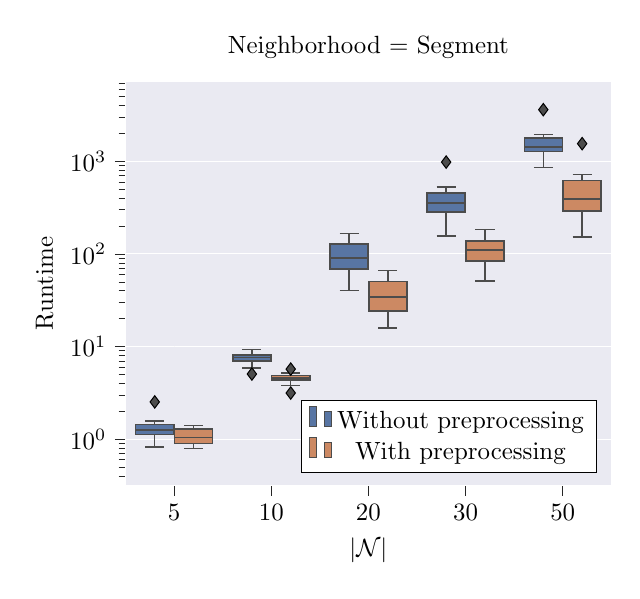
\begin{tikzpicture}[scale=0.9]

\definecolor{color0}{rgb}{0.917647058823529,0.917647058823529,0.949019607843137}
\definecolor{color1}{rgb}{0.347058823529412,0.458823529411765,0.641176470588235}
\definecolor{color2}{rgb}{0.798529411764706,0.536764705882353,0.389705882352941}

\begin{axis}[
axis background/.style={fill=color0},
axis line style={white},
tick align=outside,
title={Neighborhood = Segment},
x grid style={white},
xtick pos = left,
ytick pos = left,
xlabel={$|\mathcal N|$},
% xmajorticks=false,
xmin=-0.5, xmax=4.5,
xtick style={color=white!15!black},
xtick={0,1,2,3,4},
xticklabels={5, 10, 20, 30, 50},
y grid style={white},
ylabel={Runtime},
ymajorgrids,
% ymajorticks=false,
ymin=-0.05, ymax= 7200,
log basis y={10},
ymode = log,
ytick style={color=white!15!black},
%ytick={-0.2,0,0.2,0.4,0.6,0.8,1,1.2},
%yticklabels={−0.2,0.0,0.2,0.4,0.6,0.8,1.0,1.2},
legend pos = south east
]
\path [draw=white!29.8039215686275!black, fill=color1, semithick]
(axis cs:-0.396,1.12262684106827)
--(axis cs:-0.004,1.12262684106827)
--(axis cs:-0.004,1.43215763568878)
--(axis cs:-0.396,1.43215763568878)
--(axis cs:-0.396,1.12262684106827)
--cycle;
\path [draw=white!29.8039215686275!black, fill=color2, semithick]
(axis cs:0.004,0.893757104873657)
--(axis cs:0.396,0.893757104873657)
--(axis cs:0.396,1.28613132238388)
--(axis cs:0.004,1.28613132238388)
--(axis cs:0.004,0.893757104873657)
--cycle;
\path [draw=white!29.8039215686275!black, fill=color1, semithick]
(axis cs:0.604,7.00998145341873)
--(axis cs:0.996,7.00998145341873)
--(axis cs:0.996,8.06361049413681)
--(axis cs:0.604,8.06361049413681)
--(axis cs:0.604,7.00998145341873)
--cycle;
\path [draw=white!29.8039215686275!black, fill=color2, semithick]
(axis cs:1.004,4.35216677188873)
--(axis cs:1.396,4.35216677188873)
--(axis cs:1.396,4.86909574270249)
--(axis cs:1.004,4.86909574270249)
--(axis cs:1.004,4.35216677188873)
--cycle;
\path [draw=white!29.8039215686275!black, fill=color1, semithick]
(axis cs:1.604,68.6398023962975)
--(axis cs:1.996,68.6398023962975)
--(axis cs:1.996,127.525461196899)
--(axis cs:1.604,127.525461196899)
--(axis cs:1.604,68.6398023962975)
--cycle;
\path [draw=white!29.8039215686275!black, fill=color2, semithick]
(axis cs:2.004,24.2705239653587)
--(axis cs:2.396,24.2705239653587)
--(axis cs:2.396,50.3443903326988)
--(axis cs:2.004,50.3443903326988)
--(axis cs:2.004,24.2705239653587)
--cycle;
\path [draw=white!29.8039215686275!black, fill=color1, semithick]
(axis cs:2.604,284.469957411289)
--(axis cs:2.996,284.469957411289)
--(axis cs:2.996,456.275335729122)
--(axis cs:2.604,456.275335729122)
--(axis cs:2.604,284.469957411289)
--cycle;
\path [draw=white!29.8039215686275!black, fill=color2, semithick]
(axis cs:3.004,83.4067227244377)
--(axis cs:3.396,83.4067227244377)
--(axis cs:3.396,138.420234918594)
--(axis cs:3.004,138.420234918594)
--(axis cs:3.004,83.4067227244377)
--cycle;
\path [draw=white!29.8039215686275!black, fill=color1, semithick]
(axis cs:3.604,1276.98741739988)
--(axis cs:3.996,1276.98741739988)
--(axis cs:3.996,1779.82080817223)
--(axis cs:3.604,1779.82080817223)
--(axis cs:3.604,1276.98741739988)
--cycle;
\path [draw=white!29.8039215686275!black, fill=color2, semithick]
(axis cs:4.004,290.678902387619)
--(axis cs:4.396,290.678902387619)
--(axis cs:4.396,621.42997187376)
--(axis cs:4.004,621.42997187376)
--(axis cs:4.004,290.678902387619)
--cycle;
\path [draw=white!29.8039215686275!black, fill=color2, semithick]
(axis cs:5.004,1976.65132647753)
--(axis cs:5.396,1976.65132647753)
--(axis cs:5.396,3600.76384025812)
--(axis cs:5.004,3600.76384025812)
--(axis cs:5.004,1976.65132647753)
--cycle;
\draw[draw=white!29.8039215686275!black,fill=color1,line width=0.3pt] (axis cs:0,0) rectangle (axis cs:0,0);
\addlegendimage{ybar,ybar legend,draw=white!29.8039215686275!black,fill=color1,line width=0.3pt}
\addlegendentry{Without preprocessing}

\draw[draw=white!29.8039215686275!black,fill=color2,line width=0.3pt] (axis cs:0,0) rectangle (axis cs:0,0);
\addlegendimage{ybar,ybar legend,draw=white!29.8039215686275!black,fill=color2,line width=0.3pt}
\addlegendentry{With preprocessing}

\addplot [semithick, white!29.8039215686275!black]
table {%
-0.2 1.12262684106827
-0.2 0.822091341018677
};
\addplot [semithick, white!29.8039215686275!black]
table {%
-0.2 1.43215763568878
-0.2 1.56640148162842
};
\addplot [semithick, white!29.8039215686275!black]
table {%
-0.298 0.822091341018677
-0.102 0.822091341018677
};
\addplot [semithick, white!29.8039215686275!black]
table {%
-0.298 1.56640148162842
-0.102 1.56640148162842
};
\addplot [black, mark=diamond*, mark size=2.5, mark options={solid,fill=white!29.8039215686275!black}, only marks]
table {%
-0.2 2.52068042755127
};
\addplot [semithick, white!29.8039215686275!black]
table {%
0.2 0.893757104873657
0.2 0.788889169692993
};
\addplot [semithick, white!29.8039215686275!black]
table {%
0.2 1.28613132238388
0.2 1.40632581710815
};
\addplot [semithick, white!29.8039215686275!black]
table {%
0.102 0.788889169692993
0.298 0.788889169692993
};
\addplot [semithick, white!29.8039215686275!black]
table {%
0.102 1.40632581710815
0.298 1.40632581710815
};
\addplot [semithick, white!29.8039215686275!black]
table {%
0.8 7.00998145341873
0.8 5.85587978363037
};
\addplot [semithick, white!29.8039215686275!black]
table {%
0.8 8.06361049413681
0.8 9.2252357006073
};
\addplot [semithick, white!29.8039215686275!black]
table {%
0.702 5.85587978363037
0.898 5.85587978363037
};
\addplot [semithick, white!29.8039215686275!black]
table {%
0.702 9.2252357006073
0.898 9.2252357006073
};
\addplot [black, mark=diamond*, mark size=2.5, mark options={solid,fill=white!29.8039215686275!black}, only marks]
table {%
0.8 5.04380583763123
};
\addplot [semithick, white!29.8039215686275!black]
table {%
1.2 4.35216677188873
1.2 3.79544830322266
};
\addplot [semithick, white!29.8039215686275!black]
table {%
1.2 4.86909574270249
1.2 5.14413857460022
};
\addplot [semithick, white!29.8039215686275!black]
table {%
1.102 3.79544830322266
1.298 3.79544830322266
};
\addplot [semithick, white!29.8039215686275!black]
table {%
1.102 5.14413857460022
1.298 5.14413857460022
};
\addplot [black, mark=diamond*, mark size=2.5, mark options={solid,fill=white!29.8039215686275!black}, only marks]
table {%
1.2 3.14558386802673
1.2 5.70097041130066
};
\addplot [semithick, white!29.8039215686275!black]
table {%
1.8 68.6398023962975
1.8 40.0614998340607
};
\addplot [semithick, white!29.8039215686275!black]
table {%
1.8 127.525461196899
1.8 166.667834281921
};
\addplot [semithick, white!29.8039215686275!black]
table {%
1.702 40.0614998340607
1.898 40.0614998340607
};
\addplot [semithick, white!29.8039215686275!black]
table {%
1.702 166.667834281921
1.898 166.667834281921
};
\addplot [semithick, white!29.8039215686275!black]
table {%
2.2 24.2705239653587
2.2 15.7658724784851
};
\addplot [semithick, white!29.8039215686275!black]
table {%
2.2 50.3443903326988
2.2 66.0495994091034
};
\addplot [semithick, white!29.8039215686275!black]
table {%
2.102 15.7658724784851
2.298 15.7658724784851
};
\addplot [semithick, white!29.8039215686275!black]
table {%
2.102 66.0495994091034
2.298 66.0495994091034
};
\addplot [semithick, white!29.8039215686275!black]
table {%
2.8 284.469957411289
2.8 156.7573325634
};
\addplot [semithick, white!29.8039215686275!black]
table {%
2.8 456.275335729122
2.8 526.338541269302
};
\addplot [semithick, white!29.8039215686275!black]
table {%
2.702 156.7573325634
2.898 156.7573325634
};
\addplot [semithick, white!29.8039215686275!black]
table {%
2.702 526.338541269302
2.898 526.338541269302
};
\addplot [black, mark=diamond*, mark size=2.5, mark options={solid,fill=white!29.8039215686275!black}, only marks]
table {%
2.8 979.679989337921
};
\addplot [semithick, white!29.8039215686275!black]
table {%
3.2 83.4067227244377
3.2 50.6635050773621
};
\addplot [semithick, white!29.8039215686275!black]
table {%
3.2 138.420234918594
3.2 182.819129943848
};
\addplot [semithick, white!29.8039215686275!black]
table {%
3.102 50.6635050773621
3.298 50.6635050773621
};
\addplot [semithick, white!29.8039215686275!black]
table {%
3.102 182.819129943848
3.298 182.819129943848
};
\addplot [semithick, white!29.8039215686275!black]
table {%
3.8 1276.98741739988
3.8 855.651718139648
};
\addplot [semithick, white!29.8039215686275!black]
table {%
3.8 1779.82080817223
3.8 1954.90782356262
};
\addplot [semithick, white!29.8039215686275!black]
table {%
3.702 855.651718139648
3.898 855.651718139648
};
\addplot [semithick, white!29.8039215686275!black]
table {%
3.702 1954.90782356262
3.898 1954.90782356262
};
\addplot [black, mark=diamond*, mark size=2.5, mark options={solid,fill=white!29.8039215686275!black}, only marks]
table {%
3.8 3604.9306910038
};
\addplot [semithick, white!29.8039215686275!black]
table {%
4.2 290.678902387619
4.2 152.078605890274
};
\addplot [semithick, white!29.8039215686275!black]
table {%
4.2 621.42997187376
4.2 722.0290350914
};
\addplot [semithick, white!29.8039215686275!black]
table {%
4.102 152.078605890274
4.298 152.078605890274
};
\addplot [semithick, white!29.8039215686275!black]
table {%
4.102 722.0290350914
4.298 722.0290350914
};
\addplot [black, mark=diamond*, mark size=2.5, mark options={solid,fill=white!29.8039215686275!black}, only marks]
table {%
4.2 1548.63704776764
};
\addplot [semithick, white!29.8039215686275!black]
table {%
5.2 1976.65132647753
5.2 1663.53130054474
};
\addplot [semithick, white!29.8039215686275!black]
table {%
5.2 3600.76384025812
5.2 3601.25843000412
};
\addplot [semithick, white!29.8039215686275!black]
table {%
5.102 1663.53130054474
5.298 1663.53130054474
};
\addplot [semithick, white!29.8039215686275!black]
table {%
5.102 3601.25843000412
5.298 3601.25843000412
};
\addplot [semithick, white!29.8039215686275!black]
table {%
-0.396 1.2610787153244
-0.004 1.2610787153244
};
\addplot [semithick, white!29.8039215686275!black]
table {%
0.004 1.04564690589905
0.396 1.04564690589905
};
\addplot [semithick, white!29.8039215686275!black]
table {%
0.604 7.62893652915955
0.996 7.62893652915955
};
\addplot [semithick, white!29.8039215686275!black]
table {%
1.004 4.54212045669556
1.396 4.54212045669556
};
\addplot [semithick, white!29.8039215686275!black]
table {%
1.604 90.6794389486313
1.996 90.6794389486313
};
\addplot [semithick, white!29.8039215686275!black]
table {%
2.004 34.0904785394669
2.396 34.0904785394669
};
\addplot [semithick, white!29.8039215686275!black]
table {%
2.604 354.589285612106
2.996 354.589285612106
};
\addplot [semithick, white!29.8039215686275!black]
table {%
3.004 110.523616075516
3.396 110.523616075516
};
\addplot [semithick, white!29.8039215686275!black]
table {%
3.604 1416.90434277058
3.996 1416.90434277058
};
\addplot [semithick, white!29.8039215686275!black]
table {%
4.004 392.424636363983
4.396 392.424636363983
};
\addplot [semithick, white!29.8039215686275!black]
table {%
5.004 3135.10407328606
5.396 3135.10407328606
};
\end{axis}

\end{tikzpicture}
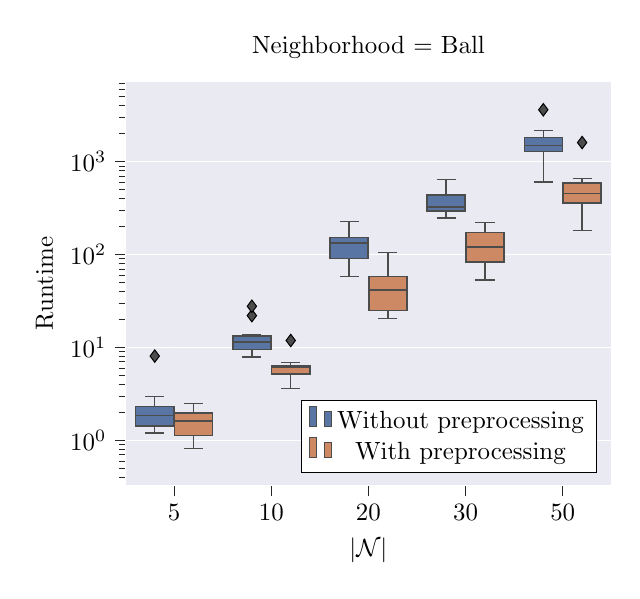
\begin{tikzpicture}[scale=0.9]

\definecolor{color0}{rgb}{0.917647058823529,0.917647058823529,0.949019607843137}
\definecolor{color1}{rgb}{0.347058823529412,0.458823529411765,0.641176470588235}
\definecolor{color2}{rgb}{0.798529411764706,0.536764705882353,0.389705882352941}

\begin{axis}[
axis background/.style={fill=color0},
axis line style={white},
tick align=outside,
title={Neighborhood = Ball},
x grid style={white},
xtick pos = left,
ytick pos = left,
xlabel={$|\mathcal N|$},
% xmajorticks=false,
xmin=-0.5, xmax=4.5,
xtick style={color=white!15!black},
xtick={0,1,2,3,4},
xticklabels={5, 10, 20, 30, 50},
y grid style={white},
ylabel={Runtime},
ymajorgrids,
% ymajorticks=false,
ymin=-0.05, ymax= 7200,
log basis y={10},
ymode = log,
ytick style={color=white!15!black},
%ytick={-0.2,0,0.2,0.4,0.6,0.8,1,1.2},
%yticklabels={−0.2,0.0,0.2,0.4,0.6,0.8,1.0,1.2},
legend pos = south east
]
\path [draw=white!29.8039215686275!black, fill=color1, semithick]
(axis cs:-0.396,1.42054045200348)
--(axis cs:-0.004,1.42054045200348)
--(axis cs:-0.004,2.29796665906906)
--(axis cs:-0.396,2.29796665906906)
--(axis cs:-0.396,1.42054045200348)
--cycle;
\path [draw=white!29.8039215686275!black, fill=color2, semithick]
(axis cs:0.004,1.13194346427917)
--(axis cs:0.396,1.13194346427917)
--(axis cs:0.396,1.95900672674179)
--(axis cs:0.004,1.95900672674179)
--(axis cs:0.004,1.13194346427917)
--cycle;
\path [draw=white!29.8039215686275!black, fill=color1, semithick]
(axis cs:0.604,9.45524632930756)
--(axis cs:0.996,9.45524632930756)
--(axis cs:0.996,13.2764401435852)
--(axis cs:0.604,13.2764401435852)
--(axis cs:0.604,9.45524632930756)
--cycle;
\path [draw=white!29.8039215686275!black, fill=color2, semithick]
(axis cs:1.004,5.14831906557083)
--(axis cs:1.396,5.14831906557083)
--(axis cs:1.396,6.28563833236694)
--(axis cs:1.004,6.28563833236694)
--(axis cs:1.004,5.14831906557083)
--cycle;
\path [draw=white!29.8039215686275!black, fill=color1, semithick]
(axis cs:1.604,90.229524075985)
--(axis cs:1.996,90.229524075985)
--(axis cs:1.996,151.581062138081)
--(axis cs:1.604,151.581062138081)
--(axis cs:1.604,90.229524075985)
--cycle;
\path [draw=white!29.8039215686275!black, fill=color2, semithick]
(axis cs:2.004,25.0485993027687)
--(axis cs:2.396,25.0485993027687)
--(axis cs:2.396,58.1326576471329)
--(axis cs:2.004,58.1326576471329)
--(axis cs:2.004,25.0485993027687)
--cycle;
\path [draw=white!29.8039215686275!black, fill=color1, semithick]
(axis cs:2.604,292.907437264919)
--(axis cs:2.996,292.907437264919)
--(axis cs:2.996,436.874851644039)
--(axis cs:2.604,436.874851644039)
--(axis cs:2.604,292.907437264919)
--cycle;
\path [draw=white!29.8039215686275!black, fill=color2, semithick]
(axis cs:3.004,82.5766415596008)
--(axis cs:3.396,82.5766415596008)
--(axis cs:3.396,172.613159298897)
--(axis cs:3.004,172.613159298897)
--(axis cs:3.004,82.5766415596008)
--cycle;
\path [draw=white!29.8039215686275!black, fill=color1, semithick]
(axis cs:3.604,1277.3001845479)
--(axis cs:3.996,1277.3001845479)
--(axis cs:3.996,1812.06858873367)
--(axis cs:3.604,1812.06858873367)
--(axis cs:3.604,1277.3001845479)
--cycle;
\path [draw=white!29.8039215686275!black, fill=color2, semithick]
(axis cs:4.004,357.813804805279)
--(axis cs:4.396,357.813804805279)
--(axis cs:4.396,585.91613727808)
--(axis cs:4.004,585.91613727808)
--(axis cs:4.004,357.813804805279)
--cycle;
\path [draw=white!29.8039215686275!black, fill=color2, semithick]
(axis cs:5.004,2533.12617921829)
--(axis cs:5.396,2533.12617921829)
--(axis cs:5.396,3600.86778354645)
--(axis cs:5.004,3600.86778354645)
--(axis cs:5.004,2533.12617921829)
--cycle;
\draw[draw=white!29.8039215686275!black,fill=color1,line width=0.3pt] (axis cs:0,0) rectangle (axis cs:0,0);
\addlegendimage{ybar,ybar legend,draw=white!29.8039215686275!black,fill=color1,line width=0.3pt}
\addlegendentry{Without preprocessing}

\draw[draw=white!29.8039215686275!black,fill=color2,line width=0.3pt] (axis cs:0,0) rectangle (axis cs:0,0);
\addlegendimage{ybar,ybar legend,draw=white!29.8039215686275!black,fill=color2,line width=0.3pt}
\addlegendentry{With preprocessing}
\addplot [semithick, white!29.8039215686275!black]
table {%
-0.2 1.42054045200348
-0.2 1.19934678077698
};
\addplot [semithick, white!29.8039215686275!black]
table {%
-0.2 2.29796665906906
-0.2 2.96406388282776
};
\addplot [semithick, white!29.8039215686275!black]
table {%
-0.298 1.19934678077698
-0.102 1.19934678077698
};
\addplot [semithick, white!29.8039215686275!black]
table {%
-0.298 2.96406388282776
-0.102 2.96406388282776
};
\addplot [black, mark=diamond*, mark size=2.5, mark options={solid,fill=white!29.8039215686275!black}, only marks]
table {%
-0.2 8.05318284034729
};
\addplot [semithick, white!29.8039215686275!black]
table {%
0.2 1.13194346427917
0.2 0.812657594680786
};
\addplot [semithick, white!29.8039215686275!black]
table {%
0.2 1.95900672674179
0.2 2.4947829246521
};
\addplot [semithick, white!29.8039215686275!black]
table {%
0.102 0.812657594680786
0.298 0.812657594680786
};
\addplot [semithick, white!29.8039215686275!black]
table {%
0.102 2.4947829246521
0.298 2.4947829246521
};
\addplot [semithick, white!29.8039215686275!black]
table {%
0.8 9.45524632930756
0.8 7.85464429855347
};
\addplot [semithick, white!29.8039215686275!black]
table {%
0.8 13.2764401435852
0.8 13.5230000019073
};
\addplot [semithick, white!29.8039215686275!black]
table {%
0.702 7.85464429855347
0.898 7.85464429855347
};
\addplot [semithick, white!29.8039215686275!black]
table {%
0.702 13.5230000019073
0.898 13.5230000019073
};
\addplot [black, mark=diamond*, mark size=2.5, mark options={solid,fill=white!29.8039215686275!black}, only marks]
table {%
0.8 21.9547684192657
0.8 27.6818652153015
};
\addplot [semithick, white!29.8039215686275!black]
table {%
1.2 5.14831906557083
1.2 3.60713505744934
};
\addplot [semithick, white!29.8039215686275!black]
table {%
1.2 6.28563833236694
1.2 6.87131643295288
};
\addplot [semithick, white!29.8039215686275!black]
table {%
1.102 3.60713505744934
1.298 3.60713505744934
};
\addplot [semithick, white!29.8039215686275!black]
table {%
1.102 6.87131643295288
1.298 6.87131643295288
};
\addplot [black, mark=diamond*, mark size=2.5, mark options={solid,fill=white!29.8039215686275!black}, only marks]
table {%
1.2 11.8492453098297
};
\addplot [semithick, white!29.8039215686275!black]
table {%
1.8 90.229524075985
1.8 58.2058568000794
};
\addplot [semithick, white!29.8039215686275!black]
table {%
1.8 151.581062138081
1.8 225.891698360443
};
\addplot [semithick, white!29.8039215686275!black]
table {%
1.702 58.2058568000794
1.898 58.2058568000794
};
\addplot [semithick, white!29.8039215686275!black]
table {%
1.702 225.891698360443
1.898 225.891698360443
};
\addplot [semithick, white!29.8039215686275!black]
table {%
2.2 25.0485993027687
2.2 20.3168349266052
};
\addplot [semithick, white!29.8039215686275!black]
table {%
2.2 58.1326576471329
2.2 104.488747596741
};
\addplot [semithick, white!29.8039215686275!black]
table {%
2.102 20.3168349266052
2.298 20.3168349266052
};
\addplot [semithick, white!29.8039215686275!black]
table {%
2.102 104.488747596741
2.298 104.488747596741
};
\addplot [semithick, white!29.8039215686275!black]
table {%
2.8 292.907437264919
2.8 246.514382123947
};
\addplot [semithick, white!29.8039215686275!black]
table {%
2.8 436.874851644039
2.8 639.965357542038
};
\addplot [semithick, white!29.8039215686275!black]
table {%
2.702 246.514382123947
2.898 246.514382123947
};
\addplot [semithick, white!29.8039215686275!black]
table {%
2.702 639.965357542038
2.898 639.965357542038
};
\addplot [semithick, white!29.8039215686275!black]
table {%
3.2 82.5766415596008
3.2 53.0783507823944
};
\addplot [semithick, white!29.8039215686275!black]
table {%
3.2 172.613159298897
3.2 219.849823713303
};
\addplot [semithick, white!29.8039215686275!black]
table {%
3.102 53.0783507823944
3.298 53.0783507823944
};
\addplot [semithick, white!29.8039215686275!black]
table {%
3.102 219.849823713303
3.298 219.849823713303
};
\addplot [semithick, white!29.8039215686275!black]
table {%
3.8 1277.3001845479
3.8 603.477584123611
};
\addplot [semithick, white!29.8039215686275!black]
table {%
3.8 1812.06858873367
3.8 2168.12077784538
};
\addplot [semithick, white!29.8039215686275!black]
table {%
3.702 603.477584123611
3.898 603.477584123611
};
\addplot [semithick, white!29.8039215686275!black]
table {%
3.702 2168.12077784538
3.898 2168.12077784538
};
\addplot [black, mark=diamond*, mark size=2.5, mark options={solid,fill=white!29.8039215686275!black}, only marks]
table {%
3.8 3605.12966704369
};
\addplot [semithick, white!29.8039215686275!black]
table {%
4.2 357.813804805279
4.2 181.127452373505
};
\addplot [semithick, white!29.8039215686275!black]
table {%
4.2 585.91613727808
4.2 658.333737373352
};
\addplot [semithick, white!29.8039215686275!black]
table {%
4.102 181.127452373505
4.298 181.127452373505
};
\addplot [semithick, white!29.8039215686275!black]
table {%
4.102 658.333737373352
4.298 658.333737373352
};
\addplot [black, mark=diamond*, mark size=2.5, mark options={solid,fill=white!29.8039215686275!black}, only marks]
table {%
4.2 1599.18166637421
};
\addplot [semithick, white!29.8039215686275!black]
table {%
5.2 2533.12617921829
5.2 1976.00723910332
};
\addplot [semithick, white!29.8039215686275!black]
table {%
5.2 3600.86778354645
5.2 3601.13235020638
};
\addplot [semithick, white!29.8039215686275!black]
table {%
5.102 1976.00723910332
5.298 1976.00723910332
};
\addplot [semithick, white!29.8039215686275!black]
table {%
5.102 3601.13235020638
5.298 3601.13235020638
};
\addplot [semithick, white!29.8039215686275!black]
table {%
-0.396 1.85927474498749
-0.004 1.85927474498749
};
\addplot [semithick, white!29.8039215686275!black]
table {%
0.004 1.61357367038727
0.396 1.61357367038727
};
\addplot [semithick, white!29.8039215686275!black]
table {%
0.604 11.3833268880844
0.996 11.3833268880844
};
\addplot [semithick, white!29.8039215686275!black]
table {%
1.004 6.04053258895874
1.396 6.04053258895874
};
\addplot [semithick, white!29.8039215686275!black]
table {%
1.604 132.37143778801
1.996 132.37143778801
};
\addplot [semithick, white!29.8039215686275!black]
table {%
2.004 41.3767584562302
2.396 41.3767584562302
};
\addplot [semithick, white!29.8039215686275!black]
table {%
2.604 325.818547606468
2.996 325.818547606468
};
\addplot [semithick, white!29.8039215686275!black]
table {%
3.004 120.167414546013
3.396 120.167414546013
};
\addplot [semithick, white!29.8039215686275!black]
table {%
3.604 1490.39417493343
3.996 1490.39417493343
};
\addplot [semithick, white!29.8039215686275!black]
table {%
4.004 451.734759449959
4.396 451.734759449959
};
\addplot [semithick, white!29.8039215686275!black]
table {%
5.004 3600.71698391438
5.396 3600.71698391438
};
\end{axis}

\end{tikzpicture}


\caption{Runtime of the model \TSPN \ without and with preprocessing when the neighborhoods are segments and balls.}
\label{fig:Fig4}
\end{figure}


\end{document}